\documentclass[11pt]{article}
\pdfoutput=1
\usepackage{jhepmod}
\usepackage{booktabs}
\usepackage[english]{babel}
\usepackage{amsmath,amssymb,amsbsy,amstext, amsthm, simplewick}
\usepackage{graphicx}
\usepackage{amsfonts}
\usepackage{mathtools}
\usepackage{amssymb}
\usepackage{upgreek}
\usepackage{listings}
\usepackage{exscale,relsize}
\usepackage[makeroom]{cancel}
\usepackage{soul}
\usepackage[utf8]{inputenc}
\RequirePackage{color}
\usepackage{amsopn, amstext, wasysym}
\usepackage{colonequals}
\usepackage{rotating}
\usepackage{multirow}
\usepackage{xspace}
\usepackage{datetime}
\usepackage[framemethod=tikz]{mdframed}
\newcommand{\db}[1]{\textcolor{green2}{(DB: #1)}}
\newcommand{\dg}[1]{\textcolor{darkgreen}{(DG: #1)}}
\newcommand{\DB}[1]{\textcolor{red}{ #1}}
\newcommand{\rp}[1]{\textcolor{blue}{#1}}
\usepackage[T1]{fontenc}
\usepackage{graphicx,scalerel}
\newmdenv[innerlinewidth=0.5pt, roundcorner=4pt,linecolor=mycolor,innerleftmargin=6pt,
innerrightmargin=6pt,innertopmargin=6pt,innerbottommargin=6pt]{mybox}

\newmdenv[innerlinewidth=0.5pt, roundcorner=4pt,linecolor=mauve,innerleftmargin=6pt,
innerrightmargin=6pt,innertopmargin=6pt,innerbottommargin=6pt]{mybox2}

\usetikzlibrary{backgrounds,fit,decorations.pathreplacing,calc}


\renewcommand{\baselinestretch}{1.14}


\definecolor{navyblue}{rgb}{0.0, 0.0, 0.9}
\definecolor{rindou1}{rgb}{0.4431,0.2862,0.7960}
\definecolor{rindou2}{rgb}{0.078,0.1215,0.4392}
\definecolor{BrickRed}{rgb}{0.0, 0.53, 0.74}
\definecolor{BlueNCS}{rgb}{0.0, 0.53, 0.74}
\definecolor{mycolor}{rgb}{0.122, 0.435, 0.698}
\definecolor{mycolor2}{rgb}{0.02, 0.435, 0.698}
\definecolor{dkgreen}{rgb}{0,0.6,0}
\definecolor{gray}{rgb}{0.5,0.5,0.5}
\definecolor{mauve}{rgb}{0.58,0.33,0.82}
\definecolor{green2}{cmyk}{0, 1, 0.5, 0}
\definecolor{lightgreen}{cmyk}{0.2, 0, 0.2, 0.2}
\definecolor{lightgray}{cmyk}{0.1,0.2,0,0.1}
\definecolor{lightgray2}{cmyk}{0.4,0.4,0,0.8}
\definecolor{black}{cmyk}{1.0,1.0,1.0,1.0}
\definecolor{celadon}{rgb}{0.67,0.88,0.69}

\lstset{frame=none,
	language=Python,
	aboveskip=1mm,
	belowskip=1mm,
	numbers=left,
	showstringspaces=false,
	columns=flexible,
	basicstyle={\ttfamily\footnotesize},
	numberstyle=\tiny\color{black},
	keywordstyle=\color{blue},
	commentstyle=\color{gray},
	stringstyle=\color{mycolor2},
	breaklines=true,
	breakatwhitespace=true,
	tabsize=3, 
	keepspaces=true
}

\newcommand{\TODO}[1]{\textcolor{red}{\textbf{#1}}}


\usepackage{amsthm}
\usepackage{upgreek}
\usepackage{slashed}
\usepackage{verbatim} 
\usepackage{scalerel}
\usepackage{lmodern}
%\usepackage[x11names]{xcolor}
\usepackage{framed}
%\colorlet{shadecolor}{LavenderBlush2} 
%\colorlet{framecolor}{Red1}
\usepackage{lipsum}
\usepackage{xcolor}
\usepackage{mathrsfs}
\usetikzlibrary{arrows}
\usepackage{colortbl}
\usepackage[framemethod=tikz]{mdframed}



\newenvironment{frshaded}{%
	\def\FrameCommand{\fboxrule=\FrameRule\fboxsep=\FrameSep \fcolorbox{framecolor}{shadecolor}}%
	\MakeFramed {\FrameRestore}}%
{\endMakeFramed}

\newenvironment{frshaded*}{%
	\def\FrameCommand{\fboxrule=\FrameRule\fboxsep=\FrameSep \fcolorbox{framecolor}{shadecolor}}%
	\MakeFramed {\advance\hsize-\width \FrameRestore}}%
{\endMakeFramed}

% Shortcuts
\def\figheight{8.9 cm}
\usepackage{pgf,tikz}
\usepackage{mathrsfs}
\usetikzlibrary{arrows}
\usepackage{placeins}
\usepackage{pgf,tikz}
\usepackage{mathtools}
\usetikzlibrary{arrows.meta}



\usepackage[utf8]{inputenc}
\usepackage[english]{babel}
\usepackage{graphicx,tipa}
\usepackage{csquotes}
\usepackage{amsmath}
\usepackage{amssymb}
\usepackage{xcolor}
\usepackage{color,wasysym}
\usepackage{bbold}
\usepackage[abs]{overpic}
\usepackage[T1]{fontenc}
\usepackage{hyperref}
\usepackage{cancel}
%\usepackage{qcircuit}
\usepackage[braket, qm]{qcircuit}
% Learn from: https://github.com/CQuIC/qcircuit/blob/master/Qtutorial.tex


%\usetikzlibrary{quantikz}


\definecolor{redred}{HTML}{D53E4F}
\newcommand{\danger}[1]{{\color{red} #1}}

\definecolor{blueblue}{HTML}{1B57B6}
\newcommand{\blue}[1]{{\color{blueblue} #1}}


\newcommand{\kp}{\ket{\psi}}
\newcommand{\bp}{\bra{\psi}}
\newcommand{\Id}{{\mathbb 1}}
\newcommand{\eS}{\mathcal{S}}
\newcommand{\mb}{\bar{m}}
\newcommand{\tm}{(\text{th})}
\newcommand{\eM}{\mathcal{M}}
\newcommand{\eN}{\mathcal{N}}
\newcommand{\eL}{\mathcal{L}}
\newcommand{\Cor}{\mathfrak{C}}
\newcommand{\Dsla}{\cancel{\mathcal{D}}}
\newcommand{\Asla}{\cancel{\mathcal{A}}}
\newcommand{\sigsla}{\cancel{\sigma}}
\newcommand{\gspa}{\mathfrak{S}}
\newcommand{\trace}{\mbox{Tr}}
\newcommand{\ie}{i.e.,~}
\newcommand{\eg}{e.g.~}
\newcommand{\T}{\texttt}
\newcommand{\PAD}{\textsc{Pandas}}
\newcommand{\QIS}{\textsc{Qiskit}}

% Make Orcid icon
\usepackage{tikz,xcolor,hyperref}
\definecolor{lime}{HTML}{A6CE39}
\DeclareRobustCommand{\orcidicon}{%
	
\begin{tikzpicture}
	\draw[lime, fill=lime] (0,0) 
	circle [radius=0.16] 
	node[white] {{\fontfamily{qag}\selectfont \tiny ID}};	\draw[white, fill=white] (-0.0625,0.095) 
	circle [radius=0.007];	\end{tikzpicture}
	\hspace{-2mm}}
\foreach \x in {A,...,Z}{%
	\expandafter\xdef\csname orcid\x\endcsname{\noexpand\href{https://orcid.org/\csname orcidauthor\x\endcsname}{\noexpand\orcidicon}}
}
\newcommand{\orcidauthorA}{0000-0003-2933-0102} %ORCID number for the author


\newcommand{\filling}{f_M}
\newcommand{\len}{\text{L}}
\usepackage{environ}
\usepackage{varwidth}
%\usepackage{showframe}
\newlength{\TheoremWidthTweak}%

\NewEnviron{short-shaded}[1][]{%
	\setlength{\TheoremWidthTweak}{\dimexpr%
		+\mdflength{innerleftmargin}
		+\mdflength{innerrightmargin}
		+\mdflength{leftmargin}
		+\mdflength{rightmargin}
	}%
	\savebox0{%
		\begin{varwidth}{\dimexpr\linewidth-\TheoremWidthTweak\relax}%
			\BODY
		\end{varwidth}%
	}%
	\begin{mdframed}[backgroundcolor=lightgray,userdefinedwidth=\dimexpr\wd0+\TheoremWidthTweak\relax, #1]
		\usebox0
	\end{mdframed}
}

\begin{document}
	\begin{titlepage}
		\setcounter{page}{1} \baselineskip=15.5pt \thispagestyle{empty}
		\bigskip\
		\vspace{1cm}
		\begin{center}
			{\fontsize{19}{38}\textsc{Notes on Data Science and Machine Learning}}  %- \large{Beginner's Guide}}}
		\end{center}
		\vspace{0.2cm}
		\begin{center}
			{\fontsize{12}{30}\selectfont Raghav G.~Jha\orcidA{}\,\footnote{\texttt{raghav.govind.jha@gmail.com}}}
		\end{center}
		
		
		\begin{center}
			\vskip 7pt
			\textsl{Thomas Jefferson National Accelerator Facility, Newport News, VA 23606, USA\\
			Perimeter Institute for Theoretical Physics, Waterloo, Ontario N2L 2Y5\\
				}
			\vskip 6pt
		\end{center}
		
		\vspace{2.6cm}
		\hrule \vspace{0.2cm}
		\noindent {\sffamily \bfseries Abstract}{ \\[0.1cm]
These notes cover some basic ideas and theory behind the field of machine learning. These notes are by no means 
even close to being exhaustive and simply meant for quick reference and interview preparation. Partly inspired by the 
amazing 100-page textbook.\footnote{The Hundred-Page Machine Learning Book. by Andriy Burkov, Quebec City, Canada, 2019}}
\vspace{0.5cm}
\hrule

\vspace{0.5cm}		
		\tableofcontents
		\vspace{0.6cm}
	\end{titlepage}
	
	
	\section{Introduction}
	
	It is no exagerration to say that all aspects of human life is related to data. 
	It is then an interesting question to ask: how much the machine can learn and think 
	like humans using that data. These questions all belong to the field of artificial intelligence (AI). 
	
	
	Machine learning (ML) originally emerged as a sub-discipline of AI research which tries to accomplish task 
	using computers without explicitly programming them. A sub-field of ML is deep learning, whose goal is to mimic
	neural networks in our brain and enable computer to function similarly. 
	
	
	What we buy, what we buy online and many others
	are all data-driven and uses machine learning (ML) methods. What movies are recommended to you on Netflix or what Amazon
	recommends you to buy in bundle are all determined by various algorithms of ML. The pricing of airline tickets and the web history 
	or what links you visit all determines what you are being shown online and how much you pay. 
	
	These notes are a brief introduction to the fundamentals and methods used in machine learning. Usually, ML is 
	classified into three parts: Supervised, Unsupervised, Reinforcement learning. The canvas of ML is shown in Fig.~\ref{fig:EXP}. 
	
	
	Machine Learning is a subfield of Data Science that deals with using existing data to help systems automatically learn new skills to perform different 	tasks without having rules to be explicitly programmed. Deep Learning, on the other hand, is a field in Machine Learning that deals with building Machine 	Learning models using algorithms that try to imitate the process of how the human brain learns from the information in a system for it to attain new 		capabilities. In Deep Learning, we make heavy use of deeply connected neural networks with many layers.
	
	
	
	
	\newpage
	\section{Some famous ML algorithms}
	
	
	

\begin{figure}
\centering 
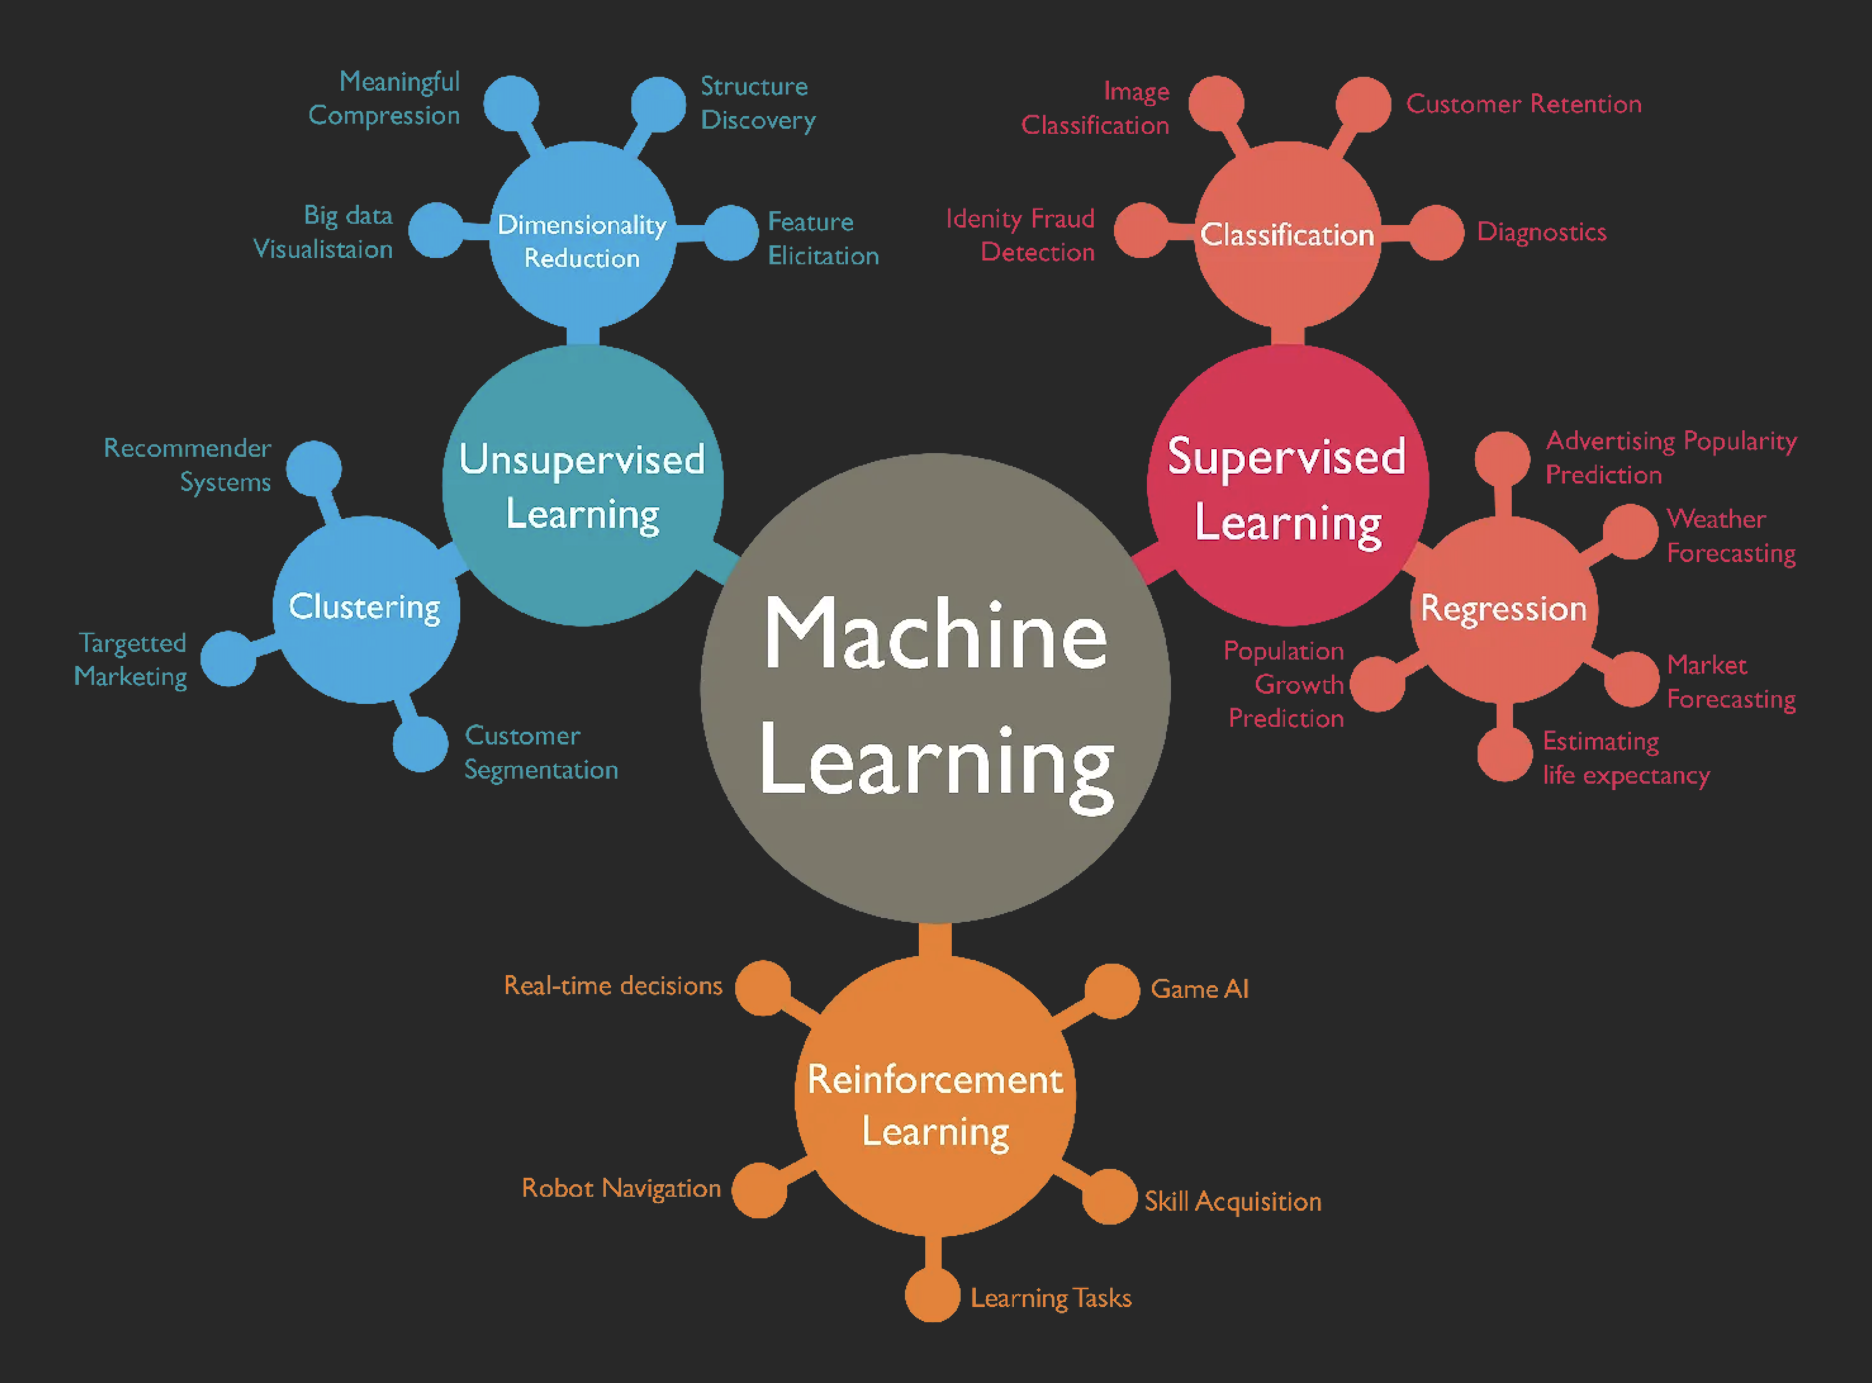
\includegraphics[width=0.65\textwidth]{cartoonML.png}
\caption{\label{fig:EXP}A cartoon showing the landscape of machine learning.}
\end{figure}
	
	
Some popular ML algorithms are: 

\begin{itemize}
\item Linear regression: This gives a relationship between input $x$ and an output variable $y$, also referred to as independent and dependent variables. 
Consider an example where you are required to arrange a few plastic boxes of different sizes on separate shelves based on their corresponding weights.
The task is to be completed without manually weighing the boxes. Instead, you need to guess the weight just by observing the height, dimensions, and sizes of the box. 
In short, the entire task is driven based on visual analysis. Thus, you have to use a combination of visible variables to make the 
final arrangement on the shelves. Linear regression in machine learning is of a similar kind, where the relationship between independent and dependent variables is established 
by fitting them to a regression line. This line has a mathematical representation given by the linear equation $y = wx + c$, where $y$ represents the dependent variable, 
$w$ = slope, $x$ = independent variable, and $b$ = intercept. We need to find the best fit by minimizing the errors using Ordinary Least Squares (OLS) as:
\begin{equation}
\text{Min.} \sum_{i=1}^{N} (y_{i} - w_{i} x_{i})
\end{equation}
\item Logistic regression: The dependent variable is of binary type (dichotomous) in logistic regression. This type of regression analysis describes data and explains the relationship between one dichotomous variable and one or more independent variables.
Logistic regression is used in predictive analysis where pertinent data predict an event probability to a logit function. Thus, it is also called logit regression.
Mathematically, logistic regression is represented by the equation:
\begin{equation}
y = \exp(b_{0} + b_{1}x)/1 + \exp(b_{0} + b_{1}x))
\end{equation}
where $x$ = input value, $y$ = predicted output, $b_0$ = bias or intercept term, $b_1$ = coefficient for input $x$.
Logistic regression could be used to predict whether a particular team will win (1) a tournament or not (0), 
or whether a lockdown will be imposed (1) due to rising COVID-19 cases or not (0) or whether a tumor is benign or not. 
Thus, the binary outcomes of logistic regression facilitate faster decision-making as you only need to pick one out of the two alternatives.
\item Decision trees: With a decision tree, you can visualize the map of potential results for a series of decisions. It enables companies to compare possible outcomes and then take a straightforward decision based on parameters such as advantages and probabilities that are beneficial to them. Decision tree algorithms can potentially anticipate the best option based on a mathematical construct and also come in handy while brainstorming over a specific decision. The tree starts with a root node (decision node) and then branches into sub-nodes representing potential outcomes. Each outcome can further create child nodes that can open up other possibilities. The algorithm generates a tree-like structure that is used for classification problems. For example, consider the decision tree below that helps finalize a weekend plan based on the weather forecast.
\item Support Vector Methods: Support vector machine algorithms are used to accomplish both classification (SVM, M for Machine) and regression (SVR, R for regression) tasks. 
With SVR, we can then give our model some flexibility in finding the predicted values, as long as the error is within that range.
In contrast to OLS discussed above in Linear regression, 
the objective function of SVR is to minimize the coefficients — more specifically, the norm of the coefficient vector — not the squared error. 
The error term is instead handled in the constraints, where we set the absolute error less than or equal to a specified margin, called the maximum error, $\epsilon$. 
We can tune epsilon to gain the desired accuracy of our model. Our new objective function and constraints are as follows:

\begin{equation}
\text{Min.} \vert \textbf{w} \vert^{2} 
\end{equation}
with contraints: $\vert y_{i} - w_{i} x_{i}\vert  \le \epsilon $. 
We can add another hyperparameter $\xi$. This is called a slack variable and the idea is simple -- for any value that falls outside of $\epsilon$, we can denote its deviation from the margin as $\xi$. 
We know that these deviations have the potential to exist, but we would still like to minimize them as much as possible. Thus, we can add these deviations to the objective function.
\begin{equation}
\text{Min.} \vert \textbf{w} \vert^{2}  + C \sum_{i=1}^{N} \vert \xi_i \vert
\end{equation}
with contraints: $\vert y_{i} - w_{i} x_{i} \vert  \le \epsilon + \vert \xi_i \vert $.
These are supervised machine learning algorithms that plot each piece of data in the $n$-dimensional space, with $n$ referring to the number of features. Each feature value is associated with a coordinate value, making it easier to plot the features. Moreover, classification is further performed by distinctly determining the hyper-plane that separates the two sets of support vectors or classes. A good separation ensures a good classification between the plotted data points. In short, SVMs represent the coordinates for individual observations. These are popular machine learning classifiers used in applications such as data classification, facial expression classification, text classification, steganography detection in digital images, speech recognition, and others.

SVM often admits the kernel trick. Kernels are used in SVM to map the original input data into a higher-dimensional space 
where it will be easier to find patterns in the data and train the model with better performance (or making the data more linear!). 
If we have binary class data like a half-moon patterns of blue and red, when plotted in 2D space, a linear SVM kernel will not be able to differentiate the two classes well but we can use RBF (radial basis function) kernel which maps the data into a particular higher-dimensional space where the two classes are clearly separable.

Typically without the kernel trick, in order to calculate support vectors and support vector classifiers, we need first to transform data points one by one to the higher dimensional space, and do the calculations based on SVM equations in the higher dimensional space, then return the results. The ‘trick’ in the kernel trick is that we design the kernels based on some conditions as mathematical functions that are equivalent to a dot product in the higher dimensional space without even having to transform data points to the higher dimensional space. i.e we can calculate support vectors and support vector classifiers in the same space where the data is provided which saves a lot of time and calculations.

%Having domain knowledge can be very helpful in choosing the optimal kernel for your problem, however in the absence of such knowledge following this default rule can be helpful: For linear problems, we can try linear or logistic kernels and for nonlinear problems, we can use RBF or Gaussian kernels.

\item Naive Bayes: This refers to a probabilistic machine learning algorithm based on the Bayesian probability model and is used to address classification problems. The fundamental assumption of the algorithm is that features under consideration are independent of each other and a change in the value of one does not impact the value of the other. For example, you can consider a ball, a cricket ball, if it is red, round, has a 7.1-7.26 cm diameter, and has a mass of 156-163 g. Although all these features could be interdependent, each one contributes to the probability that it is a cricket ball. This is the reason the algorithm is referred to as ‘naïve’. Each variable in the dataset is independent of the other. This kind of assumption is unrealistic for real-world data. However, even with this assumption, it is very useful for solving a range of complicated problems, e.g., spam email classification, etc. Let’s look at the mathematical representation of the algorithm.
If $X, Y$ = probabilistic events, $P(X)$ = probability of X being true, $P(X \vert Y)$ = conditional probability of X happening in case Y has occured. Then, Bayes’ theorem is given by the equation:
\begin{equation}
P(X \vert Y) = \frac{P(Y \vert X) P(X)}{P(Y)}
\end{equation}
A naive Bayesian approach is easy to develop and implement. It is capable of handling massive datasets and is useful for making real-time predictions. 
Its applications include spam filtering, sentiment analysis and prediction, document classification, and others.
\item kNN ($k$ Nearest Neighbor): KNN algorithm is used for both classification and regression problems. It stores all the known use cases and classifies new use cases (or data points) by segregating them into different classes. This classification is accomplished based on the similarity score of the recent use cases to the available ones. KNN is a supervised machine learning algorithm, wherein ‘K’ refers to the number of neighboring points we consider while classifying and segregating the known n groups. The algorithm learns at each step and iteration, thereby eliminating the need for any specific learning phase. The classification is based on the neighbor’s majority vote.
The algorithm uses these steps to perform the classification:
For a training dataset, calculate the distance between the data points that are to be classified and the rest of the data points.
Choose the closest ‘K’ elements based on the distance or function used.
Consider a ‘majority vote’ between the K points–the class or label dominating all data points reveals the final ranking. 
The real-life applications of KNN algorithms include facial recognition, text mining, and recommendation systems such as Amazon, Netflix, and others.
This algorithm is known as \textbf{instance-based} learning. These work by memorising the training dataset. 
The term “non-parametric” refers to not making any assumptions on the underlying data distribution. These methods do not have any fixed numbers of parameters in the model.
Similarly in KNN, the model parameters grow with the training data by considering each training case as a parameter of the model. KNN is a non-parametric algorithm.

\item $k$-Means: This is a distance-based unsupervised machine learning algorithm that accomplishes clustering tasks. In this algorithm, you classify datasets into clusters (K clusters) where the data 
points within one set remain homogenous, and the data points from two different clusters remain heterogeneous. The clusters under $k$-Means are formed using these steps:
\begin{enumerate} 
\item Initialization: The $K$-means algorithm selects centroids for each cluster (‘$K$’ number of points).
\item Assign objects to centroid: Clusters are formed with the closest centroids ($K$ clusters) at each data point.
\item Centroid update: Create new centroids based on existing clusters and determine the closest distance for each data point based on new centroids. Here, the position of the centroid also gets updated whenever required.
\item Repeat: Repeat the process till the centroids do not change.
\end{enumerate} 
K-Means clustering is useful in applications such as clustering Facebook users with common likes and dislikes, document clustering, segmenting customers who buy similar ecommerce products, etc.

Clusters are evaluated based on some similarity or dissimilarity measure such as the distance between cluster points. If the clustering algorithm separates dissimilar observations apart and similar observations together, then it has performed well. The two most popular metrics evaluation metrics for clustering algorithms are the Silhouette coefficient (S) and Dunn's index. 






\item Random forest: Random forest algorithms use multiple decision trees to handle classification and regression problems. It is a supervised machine learning algorithm where different decision trees are built on different samples during training. These algorithms help estimate missing data and tend to keep the accuracy intact in situations when a large chunk of data is missing in the dataset. Random forest algorithms follow these steps:

\begin{enumerate} 
\item Select random data samples from a given data set.
\item Build a decision tree for each data sample and provide the prediction result for each decision tree.
\item Carry out voting for each expected result.
\item  Select the final prediction result based on the highest voted prediction result.
\end{enumerate} 
This algorithm finds applications in finance, ecommerce (recommendation engines), computational biology (gene classification, biomarker discovery), and others. It uses the random subspace method, also called attribute bagging or feature bagging. It is an ensemble learning method that attempts to reduce the correlation between estimators in an ensemble by training them on \emph{random} samples of features instead of the entire feature set.

\textsc{Side Note:} Bagging is an ensemble learning method. It stands for bootstrap aggregating. In this technique, we generate some data using the bootstrap method, in which we use an already existing dataset and generate multiple samples of the $N$ size. This bootstrapped data is then used to train multiple models in parallel, which makes the bagging model more robust than a simple model. Once all the models are trained, when it’s time to make a prediction, we make predictions using all the trained models and then average the result in the case of regression, and for classification, we choose the result, generated by models, that have the highest frequency (or majority voting).



\end{itemize} 

There are primarily three different types of neural networks algorithms in deep learning (DL) that form the basis for most pre-trained models in DL:

\begin{itemize}
\item Artificial Neural Networks (ANN): Artificial neural networks are machine learning algorithms that mimic the human brain (neuronal behavior and connections) to solve complex problems. ANN has three or more interconnected layers in its computational model that process the input data. The first layer is the input layer or neurons that send input data to deeper layers. The second layer is called the hidden layer. The components of this layer change or tweak the information received through various previous layers by performing a series of data transformations. These are also called neural layers. The third layer is the output layer that sends the final output data for the problem. ANN algorithms find applications in smart home and home automation devices such as door locks, thermostats, smart speakers, lights, and appliances. They are also used in the field of computational vision, specifically in detection systems and autonomous vehicles.
\item Convolution Neural Networks (CNN): Convolutional neural networks (CNN) are all the rage in the deep learning community right now are being used across different applications and domains, and they’re especially prevalent in image and video processing projects. They mostly deal with two-dimensional objects (height and width of image). 
\item Recurrent Neural Networks (RNN): Recurrent neural networks refer to a specific type of ANN that processes sequential data. Here, the result of the previous step acts as the input to the current step. This is facilitated via the hidden state that remembers information about a sequence. It acts as a memory that maintains the information on what was previously calculated. The memory of RNN reduces the overall complexity of the neural network. RNN analyzes time series data and possesses the ability to store, learn, and maintain contexts of any length. RNN is used in cases where time sequence is of paramount importance, such as speech recognition, language translation, video frame processing, text generation, and image captioning. RNNs are a kind of feedforward network, in which information from one layer passes to another layer, and each node in the network performs mathematical operations on the data. These operations are temporal, i.e., RNNs store contextual information about previous computations in the network. It is called recurrent because it performs the same operations on some data every time it is passed. However, the output may be different based on past computations and their results.


\end{itemize} 


GNN: Graph neural networks (GNNs) to solve graph prediction tasks. A GNN is an optimizable transformation on all attributes of the graph (nodes, edges, global-context) that preserves graph symmetries (permutation invariances).


\subsection{Exploratory Data Analysis (EDA)}

EDA is a crucial step in the data science process. We can have numerical or categorical data. 
CD can further be of ordinal (size of shirt: L, XL, XXL) or nominal type (color of shirt: Blue, Green, Red). 
We can convert categorical into numerical data using two common methods: 1. Integer encoding, 
2. One-Hot Encoding. 

In integer encoding, ach unique category value is assigned an integer value.
For example, `red' is 1, `green' is 2, and `blue' is 3. This is called a label encoding or an integer encoding and is 
easily reversible. For some variables, this may be enough.
Ordinal variables like the example above would be a good example where a label encoding would be sufficient.


For categorical variables where no such ordinal relationship exists, the integer encoding is not enough.
Using this encoding and allowing the model to assume a natural ordering between categories may result in poor performance 
or unexpected results (predictions halfway between categories). In this case, a \emph{one-hot encoding} 
can be applied to the integer representation. 
This is where the integer encoded variable is 
removed and a new binary variable is added for each 
unique integer value.

In the “color” variable example, 
there are 3 categories and 
therefore 3 binary variables are needed. 
A `1' value is placed in the binary variable for the color and 
`0' values for the other colors. For example:

\begin{equation}
\begin{matrix}
Blue & Green & Red\\
1 & 0 & 0 \\
0 & 1 & 0 \\
0 & 0 & 1 
\end{matrix}
\end{equation}






\begin{mdframed}[backgroundcolor=celadon!6]
\begin{lstlisting}[language=Python]
# import necessary libraries
import pandas as pd
import numpy as np
import matplotlib.pyplot as plt
import seaborn as sns

# load the dataset
df = pd.read_csv("titanic.csv")

# print the first few rows of the DataFrame
print(df.head())

# print the DataFrame's shape
print(df.shape)

# print the DataFrame's data types
print(df.dtypes)

# check for missing values
print(df.isnull().sum())

# visualize the distribution of a numeric column
plt.hist(df['Age'])
plt.show()

# visualize the distribution of a categorical column
df['Sex'].value_counts().plot(kind='bar')
plt.show()

# calculate basic statistics for a numeric column
print(df['Fare'].describe())

# calculate the correlation between two numeric columns
print(df['Fare'].corr(df['Survived']))

# group the data by a categorical column and calculate statistics
grouped_df = df.groupby('Pclass')['Survived'].mean()
print(grouped_df)

# create a scatter plot to visualize the relationship between two numeric columns
plt.scatter(df['Age'], df['Fare'])
plt.xlabel('Age')
plt.ylabel('Fare')
plt.show()

# create a box plot to visualize the distribution of a numeric column
plt.boxplot(df['Fare'])
plt.ylabel('Fare')
plt.show()

# create a bar plot to visualize the mean of a numeric column for each category of a categorical column
df.groupby('Sex')['Age'].mean().plot(kind='bar')
plt.ylabel('Average Age')
plt.show()

# create a pivot table to summarize the data
pivot_table = df.pivot_table(index='Sex', columns='Pclass', values='Fare', aggfunc='mean')
print(pivot_table)

# create a heatmap to visualize the pivot table
plt.pcolor(pivot_table, cmap='Reds')
plt.colorbar()
plt.show()

# create a pairplot to visualize the relationships between multiple numeric columns
import seaborn as sns
sns.pairplot(df, vars=['Age', 'Fare', 'SibSp'])
plt.show()

# create a bar plot to visualize the count of a categorical column
df['Embarked'].value_counts().plot(kind='bar')
plt.ylabel('Count')
plt.show()

# create a countplot to visualize the count of a categorical column by the categories of another categorical column
sns.countplot(x='Sex', hue='Pclass', data=df)
plt.show()

# create a point plot to visualize the mean of a numeric column by the categories of a categorical column
sns.pointplot(x='Sex', y='Age', data=df)
plt.ylabel('Average Age')
plt.show()

# create a violin plot to visualize the distribution of a numeric column by the categories of a categorical column
sns.violinplot(x='Sex', y='Age', data=df)
plt.ylabel('Age')
plt.show()

# create a box plot to visualize the distribution of a numeric column by the categories of a categorical column
sns.boxplot(x='Sex', y='Age', data=df)
plt.ylabel('Age')
plt.show()

# create a swarm plot to visualize the distribution of a numeric column by the categories of a categorical column
sns.swarmplot(x='Sex', y='Age', data=df)
plt.ylabel('Age')
plt.show()

# create a faceting grid to visualize the distribution of multiple numeric columns by the categories of a categorical column
g = sns.FacetGrid(df, col='Sex')
g.map(plt.hist, 'Age')
plt.show()

# create a heatmap to visualize the correlation between multiple numeric columns
plt.figure(figsize=(12, 8))
sns.heatmap(df.corr(), cmap='RdYlGn', annot=True)
plt.show()

# create a lag plot to check for autocorrelation in a numeric column
from pandas.plotting import lag_plot
lag_plot(df['Fare'])
plt.show()

# create an autocorrelation plot to visualize the autocorrelation in a numeric column
from pandas.plotting import autocorrelation_plot
autocorrelation_plot(df['Fare'])
plt.show()

# create a scatter plot matrix to visualize the relationships between multiple numeric columns
from pandas.plotting import scatter_matrix
scatter_matrix(df[['Age', 'Fare', 'SibSp']], alpha=0.2, figsize=(6, 6))
plt.show()

# create a regression plot to visualize the relationship between two numeric columns
sns.regplot(x='Age', y='Fare', data=df)
plt.show()

# create a barplot to visualize the mean of a numeric column by the categories of a categorical column
sns.barplot(x='Sex', y='Age', data=df)
plt.ylabel('Average Age')
plt.show()

# create a pointplot to visualize the mean and confidence interval of a numeric column by the categories of a categorical column
sns.pointplot(x='Sex', y='Age', data=df, ci=95)
plt.ylabel('Average Age')
plt.show()

# create a lmplot to visualize the relationship between two numeric columns and the categories of a categorical column
sns.lmplot(x='Age', y='Fare', hue='Sex', data=df)
plt.show()

# create a factorplot to visualize the distribution of a numeric column by the categories of a categorical column
sns.factorplot(x='Sex', y='Age', data=df)
plt.ylabel('Average Age')
plt.show()

# create a boxenplot to visualize the distribution of a numeric column by the categories of a categorical column
sns.boxenplot(x='Sex', y='Age', data=df)
plt.ylabel('Age')
plt.show()

# create a distplot to visualize the distribution of a numeric column
sns.distplot(df['Fare'])
plt.show()

# create a kdeplot to visualize the kernel density estimate of a numeric column
sns.kdeplot(df['Fare'])
plt.show()

# create a rugplot to visualize the distribution of a numeric column
sns.rugplot(df['Fare'])
plt.show()

# create a jointplot to visualize the relationship between two numeric columns and their distributions
sns.jointplot(x='Age', y='Fare', data=df)
plt.show()
\end{lstlisting}
\end{mdframed}


\subsection{Data preprocessing} 


We list some steps for data preprocessing below: 

\begin{itemize} 
\item Handling missing values: This technique is used when there are missing values in the dataset. There are various ways to handle missing values, such as filling them with the mean, median, or mode of the column, or dropping rows with missing values. The appropriate method will depend on the specific dataset and the goal of the analysis.
\item Encoding categorical variables: This technique is used when the dataset contains categorical variables, which are variables that can take on a limited number of categories. One-hot encoding is a common method for encoding categorical variables, which creates a new binary column for each category. This is useful for inputting categorical variables into machine learning models, which typically only accept numerical input.
\item Standardizing numeric columns: This technique is used to scale the values of a numeric column so that they have zero mean and unit variance. This is often useful when the numeric columns have different scales and the machine learning model will be sensitive to this difference in scales.
\item Normalizing numeric columns: This technique is used to scale the values of a numeric column so that they have a minimum value of 0 and a maximum value of 1. This is often useful when the numeric columns have different scales and the machine learning model will be sensitive to this difference in scales.
\item Binning numeric columns: This technique is used to divide the values of a numeric column into bins. This is useful for turning a continuous numeric column into a categorical column, which can be useful for certain types of analysis or machine learning models.
\item Applying min-max scaling: This technique is used to scale the values of a numeric column so that they have a minimum value of 0 and a maximum value of 1. This is often useful when the numeric columns have different scales and the machine learning model will be sensitive to this difference in scales.
\item Applying robust scaling: This technique is used to scale the values of a numeric column using the median and interquartile range. This is often useful when the data contains outliers, as it is less sensitive to the influence of outliers compared to other scaling methods.
\item Applying power transformations: Power transformations are a class of functions that can be used to transform the values of a numeric column in order to stabilize or improve the assumptions of certain statistical models. Power transformations can be useful for correcting the skewness of a distribution, as skewed distributions can cause problems when fitting certain types of models.
\item Applying quantile transformations: This technique is used to transform the values of a numeric column so that they have a uniform or normal distribution. This can be useful for improving the assumptions of certain machine learning models, which may assume that the predictor variables are normally distributed.
\item Applying box-cox transformations: This technique is used to transform the values of a numeric column so that they are approximately normally distributed. This can be useful for improving the assumptions of certain machine learning models, which may assume that the predictor variables are normally distributed.
\end{itemize} 


\begin{mdframed}[backgroundcolor=celadon!6]
\begin{lstlisting}[language=Python]
# create a copy of the original DataFrame
df_preprocessed = df.copy()

# handle missing values in the DataFrame
df_preprocessed['Age'].fillna(df_preprocessed['Age'].median(), inplace=True)
df_preprocessed.dropna(inplace=True)

# encode categorical variables using one-hot encoding
df_preprocessed = pd.get_dummies(df_preprocessed, columns=['Sex', 'Pclass'], prefix=['sex', 'pclass'])

# standardize the values of a numeric column
from sklearn.preprocessing import StandardScaler

scaler = StandardScaler()
df_preprocessed['Age_scaled'] = scaler.fit_transform(df_preprocessed[['Age']])

# normalize the values of a numeric column
from sklearn.preprocessing import Normalizer

normalizer = Normalizer()
df_preprocessed['Age_normalized'] = normalizer.fit_transform(df_preprocessed[['Age']])

# bin the values of a numeric column
from sklearn.preprocessing import KBinsDiscretizer

discretizer = KBinsDiscretizer(n_bins=3, encode='ordinal')
df_preprocessed['Age_binned'] = discretizer.fit_transform(df_preprocessed[['Age']])

# apply a min-max scaling to a numeric column
from sklearn.preprocessing import MinMaxScaler

scaler = MinMaxScaler()
df_preprocessed['Age_scaled'] = scaler.fit_transform(df_preprocessed[['Age']])

# apply a robust scaling to a numeric column
from sklearn.preprocessing import RobustScaler

scaler = RobustScaler()
df_preprocessed['Age_scaled'] = scaler.fit_transform(df_preprocessed[['Age']])

# apply a power transformation to a numeric column
from sklearn.preprocessing import PowerTransformer

transformer = PowerTransformer(method='yeo-johnson')
df_preprocessed['Age_transformed'] = transformer.fit_transform(df_preprocessed[['Age']])

# apply a quantile transformation to a numeric column
from sklearn.preprocessing import QuantileTransformer

transformer = QuantileTransformer(output_distribution='normal')
df_preprocessed['Age_transformed'] = transformer.fit_transform(df_preprocessed[['Age']])

# apply a box-cox transformation to a numeric column
from scipy.stats import boxcox

df_preprocessed['Age_transformed'], lambda_ = boxcox(df_preprocessed['Age'])
\end{lstlisting}
\end{mdframed}






What is Deep Learning?

Deep learning uses artificial neural networks to perform sophisticated computations on large amounts of data. It is a type of machine learning that works based on the structure and function of the human brain. 

Deep learning algorithms train machines by learning from examples. Industries such as health care, eCommerce, entertainment, and advertising commonly use deep learning.


A neural network is structured like the human brain and consists of artificial neurons, also known as nodes. These nodes are stacked next to each other in three layers:
The input layer, the hidden layer(s), the output layer



Here is the list of top 10 most popular deep learning algorithms:
\begin{enumerate}
\item Convolutional Neural Networks (CNNs)
\item Long Short Term Memory Networks (LSTMs)
\item Recurrent Neural Networks (RNNs)
\item Generative Adversarial Networks (GANs)
\item Radial Basis Function Networks (RBFNs)
\item Multilayer Perceptrons (MLPs)
\item Self Organizing Maps (SOMs)
\item Deep Belief Networks (DBNs)
\item Restricted Boltzmann Machines( RBMs)
\item Autoencoders
\end{enumerate} 

Long Short Term Memory networks – usually just called `LSTMs' – are a special kind of RNN, 
capable of learning long-term dependencies. 
They were introduced by Hochreiter \& Schmidhuber (1997), 
and were refined and popularized by many people in following work.
They work tremendously well on a large variety of problems, and are now widely used.




Types of problems: Regression, Classification, Clustering 

\begin{enumerate}
\item Classification: Logistic regression, k-NN, Support Vector Machine (SVM), Naive Bayes, Decision Tree, Random Forest Classifiers
\item Regression: Linear (Linear, Lasso, ..), Polynomial Regression, Support Vector Regression (SVR), Decision Tree Regression, Random Forest Regression
\item Clustering: These are unsupervised algorithms. k-Means Clustering (KMC), Hierarchical Clustering (HC)
\end{enumerate}

The two clustering models have their own pros and cons. For example, the pros of k-means is that it is \emph{simple to understand, easily adaptable, works well on small or large datasets, fast, efficient and performant}
while the cons is \emph{choice of number of cluster is crucial, though can be optimally selected}.
The pros of HC is the fact that the \emph{optimal number of clusters can be obtained by the 
model itself, practical visualisation with the dendrogram}. The drawback is that it is \emph{not appropriate for large datasets}. 
These can be done using following commands: \texttt{import scipy.cluster.hierarchy as sch, dendrogram = sch.dendrogram(sch.linkage(X, method = 'ward'))}. 
Fitting HC to the dataset can be achieved by: \texttt{from sklearn.cluster import AgglomerativeClustering}



Unsupervised learning can be divided into three parts: Clustering, Dimensional Reduction based on Principal Component Analysis (PCA), and Association Problems. 
Association problems are based on identifying sequences: such as what clothes do I wear together?


Principal Component Analysis (PCA) can be 
thought of as fitting a $p$-dimensional ellipsoid to the data, 
where each axis of the ellipsoid represents a principal component. 
If some axis of the ellipsoid is small, then the variance along that axis is also small.
PCA is defined as an orthogonal linear transformation that transforms the data to a 
new coordinate system such that the greatest variance by some scalar projection of the 
data comes to lie on the first coordinate (called the first principal component), the second greatest variance on the second coordinate, and so on. 
It is method for feature extraction. 


Logistic regression is a classification algorithm traditionally limited to only two-class classification problems.
If you have more than two classes then LDA (Linear Discriminant Analysis) is the preferred linear classification technique.



PCA is an unsupervised learning algorithm while LDA is a supervised learning algorithm. 
This means that PCA finds directions of maximum variance regardless of class labels while LDA finds directions of maximum class separability.


LDA makes some assumptions as below: 
\begin{itemize} 
\item The data is Gaussian, that each variable is is shaped like a bell curve when plotted.
\item Each attribute has the same variance, that values of each variable vary around the mean by the same amount on average.
\end{itemize} 
LDA makes predictions by estimating the probability that a new set of inputs belongs to each class. The class that gets the highest probability is the output class and a prediction is made.
The model uses Bayes Theorem to estimate the probabilities.

Some extensions of LDA 

\begin{itemize} 
\item Quadratic Discriminant Analysis (QDA): Each class uses its own estimate of variance (or covariance when there are multiple input variables).
\item Flexible Discriminant Analysis (FDA): Where non-linear combinations of inputs is used such as splines.
\item Regularized Discriminant Analysis (RDA): Introduces regularization into the estimate of the variance (actually covariance), moderating the influence of different variables on LDA.
%The original development was called the Linear Discriminant or Fisher’s Discriminant Analysis. The multi-class version was referred to Multiple Discriminant Analysis. These are all simply referred to as Linear Discriminant Analysis now.
\end{itemize} 

Closely related idea if that of KPCA (kernel principal component analysis) which is nonlinear dimension reduction method. 
This transforms the data that is not linearly separable onto a new, lower-dimensional subspace that is suitable for linear classifiers. 
In Scikit-learn, it can be called as: $\texttt{from sklearn. decomposition import KernelPCA}$



\begin{mdframed}[backgroundcolor=celadon!6]
\begin{lstlisting}[language=Python]
from sklearn.discriminant_analysis import LinearDiscriminantAnalysis as LDA
sklearn_lda = LDA(n_components=2)
X_lda_sklearn = sklearn_lda.fit_transform(X, y)
\end{lstlisting}
\end{mdframed}



\begin{mdframed}[backgroundcolor=celadon!6]
\begin{lstlisting}[language=Python]
import numpy as np
from sklearn.decomposition import PCA
X = np.array([[-1, -1], [-2, -1], [-3, -2], [1, 1], [2, 1], [3, 2]])
pca = PCA(n_components=2)
pca.fit(X)
PCA(n_components=2)
print(pca.explained_variance_ratio_)
print(pca.singular_values_)
\end{lstlisting}
\end{mdframed}


Between supervised and unsupervised learning, we have something which is - reinforcement learning (RL). 
It is the case where we have no data at all, like city for a self-driven car. In this sense, the entire
knowledge about roads and traffic rules won't teach the car how to drive itself. The goal is to minimize errors
and not to predict the moves! Survival of the fittest or rather the algorithm is the sole motive of RL. 

Q-learning is a commonly used model-free approach which can be used for building a self-playing PacMan agent. 
It revolves around the notion of updating Q values which denotes value of performing action a in state $s$. 
The following value update rule is the core of the Q-learning algorithm.



\subsection{Data cleaning}

It is part of  Data wrangling which includes  importing, cleaning, structuring, handling missing values, text mining. 

It is important aspect of data science and can be summarised below in some steps:

\begin{itemize}
\item Missing Values: Identify missing values in the dataset. Decide on an appropriate method to handle missing values, such as imputation or deletion. 
Impute missing values with appropriate values based on the method selected, such as mean, median, or mode. 
In \PAD~we can use: $\texttt{df.isna()}$ and $\texttt{df.isna().sum()}$ to check which enteries are not available. 

Alternatively, for mean imputation we can use:
in \PAD -- $\texttt{df.fillna(df.mean())}$


\begin{mdframed}[backgroundcolor=celadon!6]
\lstinputlisting[language=Python]{codes/f_mv.py}
\end{mdframed}



\item Duplicates: Identify and remove duplicate records in the dataset. Verify that all duplicates have been removed
\item Outliers: Identify and handle outliers or extreme values in the data Decide on an appropriate method to handle outliers, such as deletion, transformation, or imputation. Impute or delete outliers based on the method selected such as RANSAC
\item Data Format: Verify that all data is in the correct format. Convert data into the appropriate format, such as converting dates into a common format. Handle inconsistent data formats\
\item Data Validity: Verify all data is valid and consistent. Check for errors (incorrect values or typos) and correct them
\item Data Standardization and Normalization: Data is generally processed in one of two ways:  data standardization or data normalization, sometimes referred to as min-max scaling. The two most popular techniques for scaling numerical data prior to modeling are normalization and standardization. Normalization scales each input variable separately to the range 0-1, which is the range for floating-point values where we have the most precision. Standardization scales each input variable separately by subtracting the mean (called centering) and dividing by the standard deviation to shift the distribution to have a mean of zero and a standard deviation of one. This can be achieved in \PAD~as 
\end{itemize}





\begin{figure}
\centering 
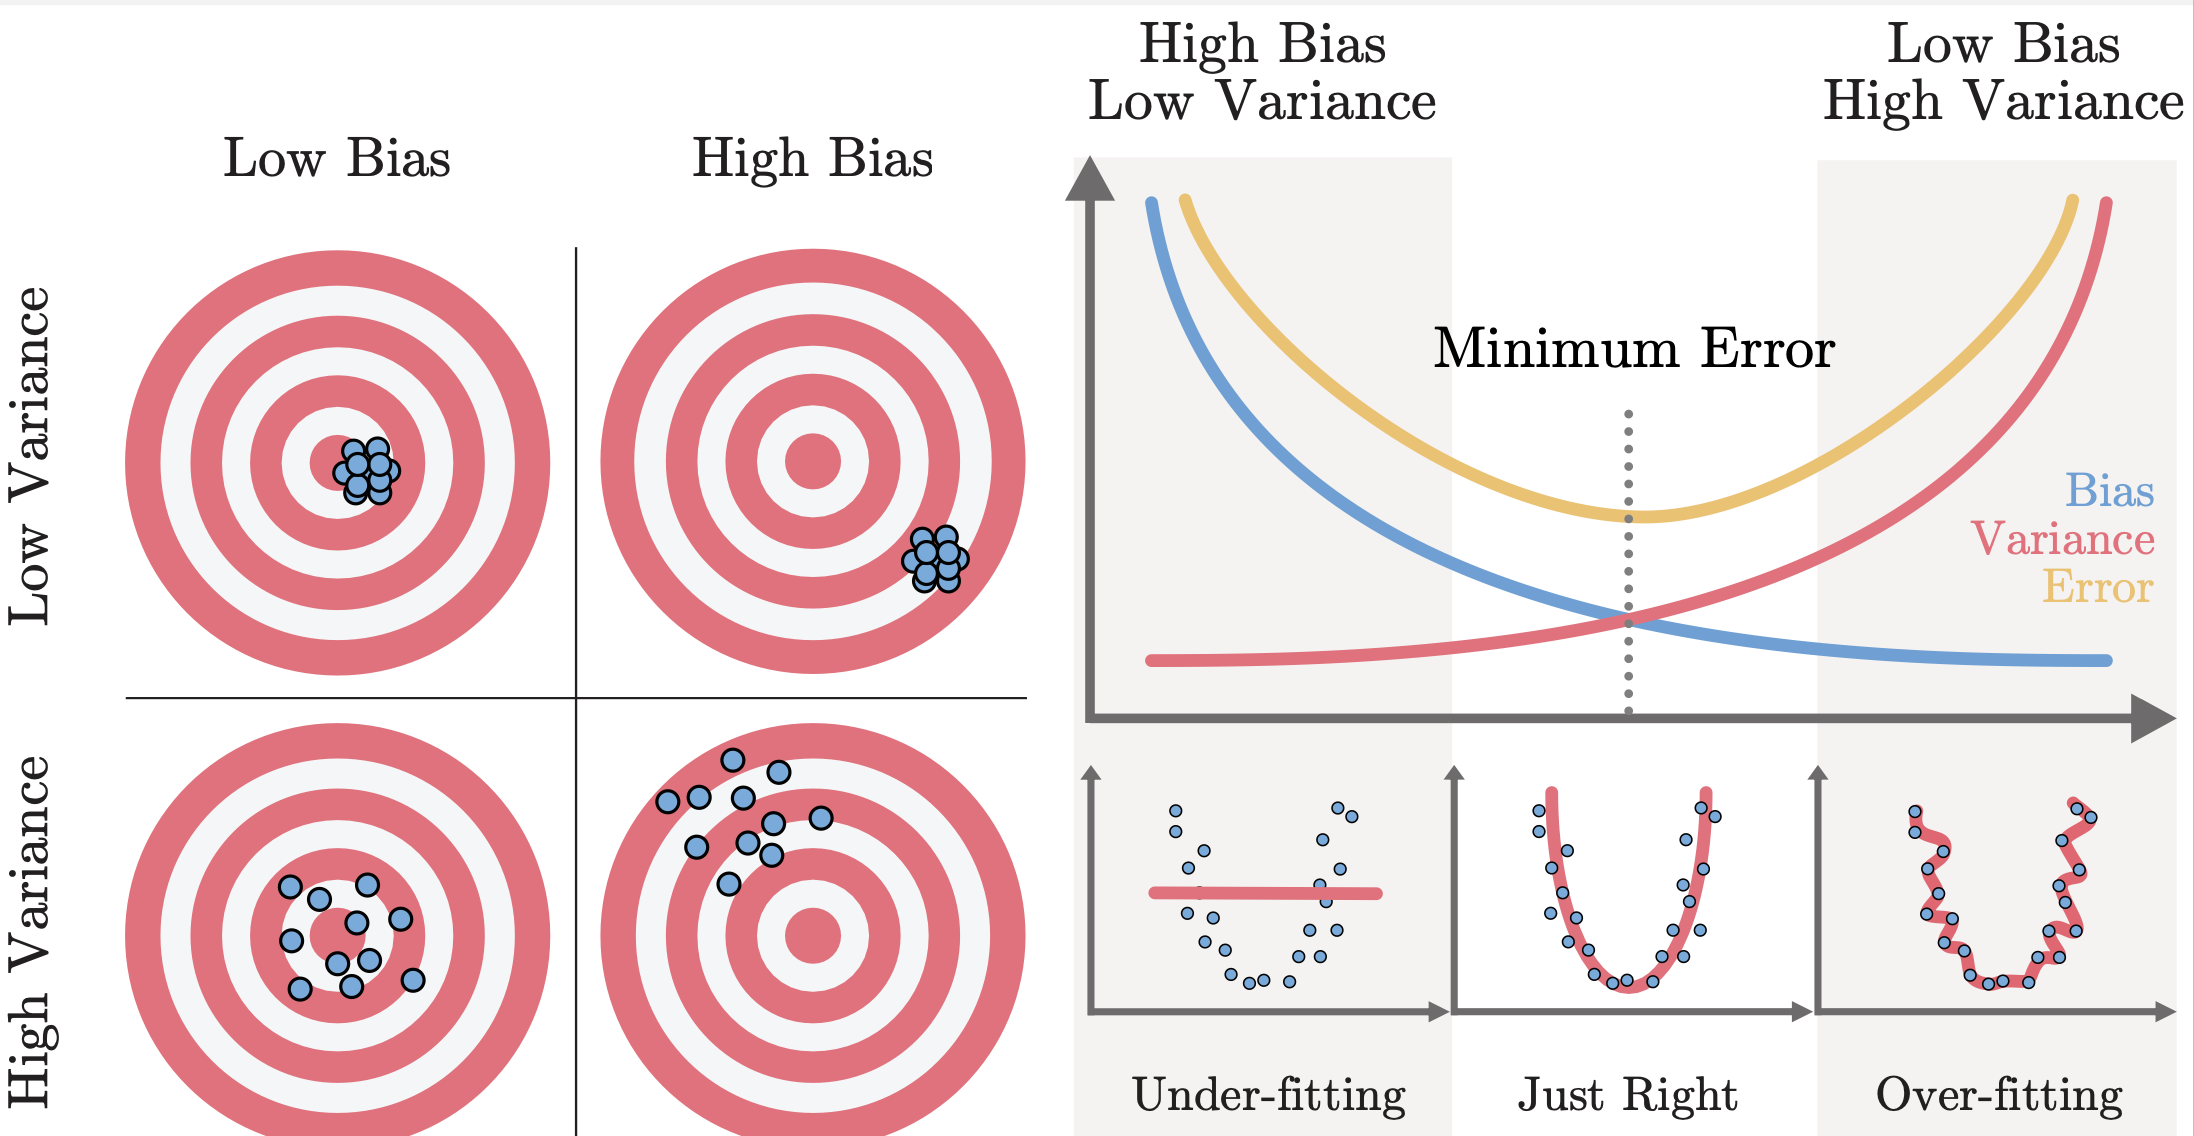
\includegraphics[width=0.65\textwidth]{cartoon1.png}
\caption{\label{fig:bias1}Diagrammatic representation of bias and variance and how we can over/under fit the model.}
\end{figure}


\section{Definitions:}


In $k$-fold cross-validation, 
we divide the dataset into $k$ equal parts. 
After this, we loop over the entire dataset $k$ times. 
In each iteration of the loop, one of the $k$ parts is used for testing, 
and the other $k-1$ parts are used for training. 
Using $k$-fold cross-validation, each one 
of the $k$ parts of the dataset ends up 
being used for training and testing purposes.
An improvement of this is stratified $k$-fold cross-validation. 

A special case of $k$-fold cross-validation is LOOCV (leave-one-out cross-validation)
where we do not leave one training set for test but rather choose $k=n$ so that only one training example is
used for testing during each iteration. 

%\texttt{from sklearn.model_selection import GridSearchCV} followed by 
%\texttt{GridSearchCV(estimator=SVC(),param_grid={'C': [1, 10], 'kernel': ('linear', 'rbf')})}


\subsection{Confusion matrix}

A matrix that lays out the performance of a learning algorithm. 
It has four elements, \textbf{TP} (true positive),  \textbf{TN} (true negative), 
\textbf{FP} (false positive) and \textbf{FN} (false negative). 

\begin{equation}
\textbf{ERR} = \frac{FP+FN}{FP+FN+TP+TN} 
\end{equation}

whereas the prediction accuracy is 1-ERR. We also have FPR, TPR. 

\begin{equation}
\textbf{FPR} = \frac{FP}{FP+TN}  = 1 - \textbf{TNR} 
\end{equation}

\begin{equation}
\textbf{TPR} = \frac{TP}{FN+TP} 
\end{equation}

REC (recall) is equal to TPR while PRE (precision) is defined as:
\begin{equation}
\textbf{PRE} = \frac{TP}{FP+TP} 
\end{equation}

All same meaning: [Sensitivity, Recall, Hit rate, or True positive rate] and [Specificity, Selectivity or True negative rate (TNR)]


F1 score is the harmonic mean of \textbf{PRE} and \textbf{REC}, and it is calculated 
using the following formula: 
\[ F1 = \frac{2 \cdot \textbf{PRE} \cdot \textbf{REC}}{\textbf{PRE} + \textbf{REC}}\] 
The F1 score is used when the recall and the precision are equally important.




\subsection{Stochastic Gradient Descent (SGD)} 


In several problems in machine learning, we have to optimize. The optimizer is an algorithm that adjusts the weights to minimize the loss. Nearly 
all of the optimization algorithms used in deep learning belong to a family called stochastic gradient descent. 
They are iterative algorithms that train a network in steps. One step of training goes is as follows:

\begin{itemize}
\item Sample some training data and run it through the network to make predictions.
\item Measure the loss between the predictions and the true values.
\item Adjust the weights in a direction that makes the loss smaller.
\end{itemize} 


An astute reader might ask: why is it called SGD? 
It is called so because, the gradient is a vector that specifies in what direction the weights need to move. 
More precisely, it tells us how to change the weights to make the loss change fastest. We call our process 
gradient descent because it uses the gradient to descend the loss curve towards a minimum. Stochastic means 
`determined by chance'. Our training is stochastic because the batches we use 
are random samples from the dataset. Hence, the name SGD. 


\begin{itemize} 
\item Overfitting: The model captures the training data well but fails to generalize to unseen data. High variance, Low bias. 
\item Underfitting: The model does not capture the training data well. High variance, high bias. 
\end{itemize} 


We define variance as measure of how much deviation occurs for particular case if we retrain the model
multiple times using different subsets of training data. 

\textbf{How to reduce overfitting}

We can either do regularization or \emph{dimensional reduction via feature selection}. 


\subsection{Activation function} 

An activation function is a function used in artificial neural networks which outputs a small value for small inputs, and a larger value if the 
inputs exceed a threshold. If the inputs are large enough, the activation function "fires", 
otherwise it does nothing. In other words, an activation function is like a gate 
that checks that an incoming value is greater than a critical number.

Activation functions are useful because they add non-linearities into neural networks, 
allowing the neural networks to learn powerful operations. 
If the activation functions were to be removed from a feedforward neural network, 
the entire network could be re-factored to a simple linear operation or matrix transformation on its input, 
and it would no longer be capable of performing complex tasks such as image recognition.
\emph{A neural network with no activation functions is equivalent to a linear regression model, and can perform no operation more complex than linear modeling}.

Well-known activation functions used in data science include the rectified linear unit (ReLU) function, 
and the family of sigmoid functions such as the logistic sigmoid function, 
the hyperbolic tangent, and the arctangent function.
Two commonly used activation functions: the rectified linear unit (ReLU) and the logistic sigmoid function. The ReLU has a hard cutoff at 0 where 
its behavior changes, while the sigmoid exhibits a gradual change. Both tend to 0 for small $x$, and the sigmoid tends to 1 for large $x$.

\subsubsection{ReLU derivative} 

\begin{equation} 
f(x)=
\begin{cases} 
0 & \text{if  }  x < 0 \\
1 & \text{if  }  x > 0 \\
\end{cases}
\end{equation} 
The reason for it being undefined at $x=0$ is that its left- and right derivative are not equal. 
This sometimes creates problem with `backpropagation' since 
when training a neural network, a neuron can become `trapped' in the zero region 
and backpropagation will never change its weights. Because of the zero gradient problem faced by the ReLU, 
it is sometimes common to use an adjusted ReLU function called the parametric rectified linear unit, or PReLU:
\begin{equation} 
f(\alpha, x)=
\begin{cases} 
x & \text{if  }  x \ge 0 \\
\alpha x & \text{if  }  x < 0 \\
\end{cases}
\end{equation} 
This has the advantage that the gradient is nonzero at all points (except 0 where it is undefined).


\begin{equation} 
f(x) = \dfrac{\exp(x)}{1+\exp(x)} = \dfrac{1}{1+\exp(-x)}
\end{equation} 



\subsection{Back propagation} 


Backpropagation can be thought of 
as a computationally efficient approach to 
compute the partial derivatives of a complex cost function
in multilayer NNs. The challenge in the parameterization of NN
is that we are typically dealing with a very large number of weight coefficients in a 
high-dimensional feature space. In contrast to cost functions of single-layer NNs such as 
Adaline (single layer), which we have seen in previous chapters, the error 
surface of an NN cost function is not convex or smooth with respect to the parameters. 
There are many bumps in this high-dimensional cost surface (local minima) 
that we have to overcome in order to find the global minimum of the cost function.

Automatic differentiation comes with two modes, the forward and reverse modes.
Backpropagation is simply a special case of reverse-mode automatic differentiation.
The trick of reverse mode is that we start from right to left: we multiply a matrix by a vector, 
which yields another vector that is multiplied by the next matrix and so on. 
Matrix-vector multiplication is computationally much cheaper than matrix-matrix multiplication, 
which is why backpropagation is one of the most popular algorithms used in NN training.


We start by computing:

\begin{itemize}
\item $textbf \delta^{\rm{out}}  = \textbf{a}^{\rm{out}} - \textbf{y}$
\end{itemize}
where $\textbf{y}$ is the vector of true class labels. Now, we compute error in the hidden layer as:


\begin{equation}
textbf{\delta}^{\rm{(h)}} = textbf{\delta}^{\rm{out}} \Big( \textbf{W}^{\rm{out}}\Big)^{T} \otimes \frac{\partial \phi(z^{(h)})}{\partial z^{(h)}}  
\end{equation}
where derivative is taken of the activation function (sigmoid etc.)  



\TODO{Fill in .....} 




\section{Quantum meets Machine Learning = QML} 

The idea of QML was first introduced in \cite{2013arXiv1307.0411L}. 
We would not talk about unsupervised QML or quantum reinforcement learning and will only 
make note of supervised QML. 


Check out - \href{https://github.com/Qiskit/qiskit-machine-learning}{QISKIT ML}  \\ 
\href{https://github.com/tensorflow/quantum}{TensorFlow Quantum}  \cite{2020arXiv200302989B}  \\ 
And of course, we have \textsc{Penny Lane} developed at Xanadu by Schuld et al. 

\subsection{Acronyms used in QML} 

\begin{itemize}
\item QNNA: Quantum nearest-neighbor algorithm 
\item QDTC: Quantum decision tree classifiers
\item QKM: Quantum kernel methods
\item QSVM: Quantum support vector machines
\item QNNC: Quantum neural network classifiers
\end{itemize}

In QML, we have two data encoding methods. Amplitude encoding (AE) and block encoding (BE). 

\begin{itemize}
\item AE: The data vector is encoded in the amplitude of the quantum state and then passed to quantum neural network. 
A $2^{n}$-dimensional vector can be encoded in $n$ qubits as is well-known. AE based QNNs are regarded as 
`kernel methods' \footnote{Kernel methods owe their name to the use of kernel functions (positive-definite kernel or kernel function is a generalization of a positive-definite function or a positive-definite matrix.), 
which enable them to operate in a high-dimensional, implicit feature space without ever computing the coordinates of the data in that space, but rather by simply computing the inner products between the images of all pairs of data in the feature space.}. Encoding is a very important step! It is often a bottleneck for the runtime. 
\item BE: This is more practical on NISQ devices. The initial quantum state is fixed and 
the input data is required to be encoded into the QNN circuit classically in a way similar to the encoding of the variational parameters.
There is no need for QRAM (quantum RAM). 
\end{itemize}

For QML, we need to remember that there are some conditions on the 
preprocessing i.e., unit length of input vector which is because of the normalized state. 
The result of QML is a measurement made by the observer. 



\TODO{By May 2023!} 

\TODO{Tensor networks for QML}

One of the interesting things is whether we can use the idea of tensor networks 
to understand QML better. Much work has been done and a good reference page is 
\href{https://tensornetwork.org/ml/}{this}. I suspect that there should already be work on encoding using these structures. 

%\section{Acknowledgements}



\appendix  

\section{Some probability recap} 

\textsc{Question 1:} What is the probability to get two heads consecutively when a coin is tossed 5 times. What about general $n$? \\ \\ 
\textsc{Question 2:} Suppose $P(A)$ is the probability that $A$ passes an exam, $P(B)$ is the probability that $B$ passes an exam, $P(A \cap B)$ is that both passes, $P(A \cup B)$ is at least one passes. We have: 
\[ P(A \cup B) = P(A) + P(B) - P(A \cap B) \] 

% https://www.geeksforgeeks.org/expected-number-of-trials-to-get-n-consecutive-heads/?ref=rp



\section{Some statistics recap}

\begin{itemize}
\item Central limit theorem: According to CLT, we can treat sampling distribution of any population as normal irrespective of the distribution function of the 
population. This theorem needs the sample size to be large enough.
\item R-squared ($R^2$) is a statistical measure that represents the proportion of the variance for a dependent variable that's explained by an independent variable or variables in a regression model. $R^2 = 1$ means that all variation in dependent can be explained. R-Squared only works as intended in a simple linear regression model with one explanatory variable. With a multiple regression made up of several independent variables, the R-Squared must be adjusted.
The adjusted R-squared compares the descriptive power of regression models that include diverse numbers of predictors. Every predictor added to a model increases R-squared and never decreases it. Thus, a model with more terms may seem to have a better fit just for the fact that it has more terms, while the adjusted R-squared compensates for the addition of variables and only increases if the new term enhances the model above what would be obtained by probability and decreases when a predictor enhances the model less than what is predicted by chance. In an overfitting situation, 
an incorrectly high value of R-squared is obtained, even when the model actually has a decreased ability to predict. This is not the case with the adjusted R-squared.
\item $p$-value: The p-value is a probability that the observed spatial pattern was created by some random process. When the $p$-value is very small i.e., $ p < 0.05$, it means it is very unlikely that the observed spatial pattern is the result of random processes, so you can reject the null hypothesis.\
In other words, \emph{a $p$-value is a number describing how likely it is that your data would have occurred under the null hypothesis of your statistical test.}
The $p$ value can only tell you whether or not the null hypothesis is supported. It cannot tell you whether your alternative hypothesis is true, or why.
The threshold value for determining statistical significance is also known as the $\alpha$-value. All statistical tests have a null hypothesis. For most tests, the null hypothesis is that there is no relationship between your variables of interest or that there is no difference among groups. For example, in a $t$ test, the null hypothesis is that the difference between two groups is zero. Recall that a 
$t$-test is a statistical test that is used to compare the means of any two groups. 
\item $z$-score: $z$-scores are standard deviations. For example a $z=2$ means that the result is 2 standard deviations from the mean. 
Both $z$-scores and $p$-values are associated with the standard normal distribution. Very high or very low (negative) $z$-scores, 
associated with very small $p$-values, are found in the tails of the normal distribution. The higher or lower the $z$-score, the more unlikely the result is to happen by chance and the more likely the result is meaningful.
\end{itemize}  

\section{Recommender Systems}

A recommender system (RS), or a recommendation system, is a subclass of information filtering system that seeks to predict the “rating” or “preference” a user would give to an item. Recommender systems are utilized in a variety of areas, with commonly recognized examples taking the form of playlist generators for video and music services, product recommenders for online stores, etc. These systems can operate using a single input, like music, or multiple inputs within and across platforms like news, books, and search queries. Recommender systems are utilized in order to make better product suggestions to customers, or personalized recommendations to friends.

RSs leverage machine learning algorithms in order to make better predictions about a user’s preferences. There are a number of different machine learning algorithms that can be used in a recommender system. Each algorithm has its own strengths and weaknesses, and the best algorithm for a particular application will depend on the nature of the data. The most common is the linear regression algorithm. The linear regression algorithm is used to find the best linear approximation to a data set. In a recommender system, this algorithm is used to predict how a user will rate an item based on their past ratings. Other machine learning algorithms that can be used in RS, include some of the following:

\begin{itemize}
\item Neural Networks: A neural network is a type of machine learning algorithm that is similar to the brain. It is composed of interconnected neurons that can learn to recognize patterns. Neural networks are often used for prediction tasks, like recommender systems.
\item K-NearestNeighbor (K-NN): The K-NN algorithm is often used for recommender systems because it is able to handle large amounts of data and can produce good predictions. The K-NN algorithm works by finding the k nearest neighbours of a given item. The neighbours are then used to vote on the rating of the item. The algorithm then uses the average of the votes to predict the rating of the item. The K-NN algorithm is often used for Recommender Systems because it is able to handle large amounts of data and can produce good predictions.
\item Bayesian inference: Bayesian inference is a type of machine learning algorithm that is used to make better predictions. It is often used in recommender systems because it can handle large amounts of data. The Bayesian inference algorithm works by using a probability model to predict the rating of an item. The algorithm uses the past ratings of a user to build the probability model. This allows the algorithm to make better predictions about a user’s preferences.
\item Dimensionality reduction: Dimensionality reduction is a type of machine learning algorithm that is used to reduce the number of dimensions in a data set. It is often used in Recommender Systems because it can help to reduce the amount of data that needs to be processed. The dimensionality reduction algorithm works by finding a lower dimensional representation of the data. This can be done by using techniques like Principal Component Analysis (PCA).These are just some of the machine learning algorithms that can be used in Recommender Systems. Each algorithm has its own strengths and weaknesses, and the best algorithm for a particular application will depend on the nature of the data.
\end{itemize}


The following is a list of benefits / value of building recommender system and why businesses must consider:

\begin{itemize}
\item Recommender systems help businesses make money by increasing sales and predicting what customers want.
\item Recommender systems can improve customer satisfaction by providing relevant recommendations. They can improve customer loyalty by suggesting new items that the customer may like.
\item Recommender systems can reduce the amount of time it takes to find the right item for a customer.
\item Recommender systems can help businesses learn more about their customers’ preferences.
\end{itemize}


There are different types of RS. Some of them are listed below:

\begin{itemize}
\item Content-based recommendation: The most common type of recommender system is the content-based recommender system. A content-based recommender system is a type of recommender system that relies on the similarity between items to make recommendations. For example, if you’re looking for a new movie to watch, a content-based recommender system might recommend movies that are similar to ones you’ve watched in the past. Content-based recommender systems are commonly used in music, books, and movies. They can be used to recommend products, services, or even websites. Content-based recommender systems are based on the idea that if you like one item, you’re likely to like other items that are similar to it. To build a content-based recommender system, you need to first define what similarity means. This is where machine learning comes in. A content-based recommender system can use machine learning to learn the similarity between items. Once it has learned the similarity between items, it can make recommendations accordingly.

\item Collaborative filtering based recommendation: 
Another type of recommender system is the collaborative filtering recommender system. A collaborative filtering recommender system is a type of machine learning algorithm that makes predictions about what a user might want to buy or watch based on the past behavior of other users. The algorithm looks at the items that other users with similar taste have purchased or rated highly, and recommends those items to the new user.
The main advantage of collaborative filtering is that it doesn’t require any information about the users or items; all it needs is a dataset of past user behavior. Collaborative filtering is one of the most popular techniques for building recommender systems, and is used by major companies such as Amazon, Netflix, and Spotify.

\item Hybrid recommender system: A third type of recommender system is the hybrid recommender system. The hybrid approach has become increasingly popular in recent years as it offers the potential to overcome some of the limitations of each individual approach.
\end{itemize}




Content-based recommender systems focus on the attributes of items in order to make recommendations. This can often lead to issues with scalability, as the system needs to be constantly updated with new content in order to make accurate recommendations. Collaborative filtering systems, on the other hand, focus on the relationships between users and items. This can often result in problems with sparsity, as it can be difficult to find enough users who have rated a given item. The hybrid approach seeks to overcome these limitations by combining the two approaches. 

A hybrid recommender system is a type of recommender system that combines both content-based and collaborative filtering approaches. The hybrid approach takes advantage of both content-based and collaborative filtering by using them to supplement each other. For example, a hybrid recommender system might first identify a set of items that are similar to the item the user is interested in, and then use collaborative filtering to identify which of those items the user is most likely to enjoy. This approach can provide more accurate recommendations than either method used alone. The hybrid approach has been shown to be more effective than either method used alone, as it is able to leverage the strengths of both approaches. Hybrid recommender systems are often more scalable and efficient than pure content-based or collaborative filtering systems.

Examples of Recommender Systems
Some of the most popular examples of recommender systems include the ones used by Amazon, Netflix, and Spotify.

Amazon’s recommender system is based on a combination of collaborative filtering and content-based algorithms. It uses past customer behavior to make recommendations for new products. Amazon’s recommender system is one of the most complex and sophisticated in the world.
Netflix’s recommender system is also based on a combination of collaborative filtering and content-based algorithms. However, Netflix takes things a step further by also incorporating machine learning into its algorithm. This allows Netflix to make predictions about what a user might want to watch based on the behavior of other users.
Spotify’s recommender system is based on collaborative filtering. It uses past user behavior to make recommendations for new songs to listen to.


In short, recommender systems are a type of machine learning based systems that are used to predict the ratings or preferences of items for a given user. There are three main types of Recommender Systems: collaborative filtering, content-based, and hybrid. Some of the most popular examples of Recommender Systems include the ones used by Amazon, Netflix, and Spotify. Collaborative filtering systems use past user behavior to make recommendations for new products. Content-based systems focus on the attributes of items in order to make recommendations. The hybrid approach is a combination of both content-based and collaborative filtering approaches. Hybrid recommender systems are often more scalable and efficient than pure content-based or collaborative filtering systems. 

In the most basic setup, the RS is made up of five core components:
as shown in Fig. below. 

\begin{enumerate}
\item Data Collection and Processing 
\item Recommender Model
\item Recommendation post-processing
\item Online modules (tells us what needs to be stored in logs in order to both report how your system is performing and perhaps to also learn from the usage and interactions)
\item User interface (For example, it’s good practice to explain to users why they are being recommended an item (e.g. `You may like watching this movie because you liked movies $X$ and $Y$), as this makes the recommender’s decisions more transparent.)
\end{enumerate} 


\subsubsection{Dithering}

There is a relatively low cost but high value technique for improving the quality of our 
recommendations known as `dithering'. It’s a technique that re-orders a list of recommendations by slightly shuffling them around based on some noise. 
It is typically implemented in the recommendation post-processing component.





\section{Natural Language Processing (NLP), ChatGPT and all that..}

Unless you have been living in the mountains with no internet, you must have read 
or experimented with ChatGPT. In this post, and probably subsequent ones, we will try to explain 
what makes it tick and the foundations behind this progress. First some acronyms used:

\begin{itemize}
\item ML: Machine learning
\item LLM: Large Language Model
\item GPT: Generative Pre-training Transformer
\item LSTM: Long-Short-Term-Memory
\end{itemize}

and Tranformer models


ChatGPT is an extrapolation of a class of ML models known as LLM. LLMs takes in 
huge quantities of text data and infer relationships between words in that text. 
The capability of LLMs increase with increase in size of their input datasets and parameter space. 


In NLP, one is interested in making inferences from large data of text. 
The most basic and traditional method was S-to-S (sequence to sequence) models. 
However, when we have large amount of text this was not optimal since the model 
forgets the learning from the earlier parts as it moves along a sequence. This means 
that there is loss of information/learning. LSTM and GRU's did try to salvage this situation 
by discarding information that was not useful along the way to remember important information. 
Though, it still wasn’t enough. Then in 2014, a paper introduced `attention mechanisms'. 
The authors suggested assigning relative importance to each word in a sentence such that the 
model focuses on important words and ignores the rest (much like importance sampling in Monte Carlo methods). 
It emerged to be a massive improvement over encoder-decoder models. 


The most basic training of language models involves predicting a word in a 
sequence of words. This is observed as either next-token-prediction (you must have noticed this in Gmail when composing an email when it suggest auto completion) 
and masked-language-modeling (where a sentence like `Bill ??? running', is suggested completion through words as `likes', `hates' etc. ??? denotes the mask!). 
These basic-sequencing techniques are often implemented through LSTM. However, it has some drawbacks! 

While running might be associated to `hate', it might be that Bill is a marathon runner and actually loves it. There might be other sentences in the text
which affirms this like `Bill runs thrice a day'. However, if it is masked, LSTM might actually assign `hate' to complete the sentence as:
`Bill hates running'. This means that the model is unable to give more importance to some surrounding words than others. 
The other issue is that the input data is processed individually and sequentially rather than as a whole big chunk. 
This means that when an LSTM is trained, the window of context is fixed. This limits the complexity of the relationships between words and the meanings that can be derived.
So, suppose we have two sentences -- `Stochastic gradient is a very powerful tool in machine learning' , and `Stochastic gradient which is related to conjugate gradient 
is a method frequently used in inverting fermionic operators in lattice field theory'. Now, if we train the model, and ask `What is stochastic gradient?'. It will not 
say anything about lattice field theory since it doesn't see the whole corpus of data. 


Because of these limitations, in 2017, a paper titled `Attention is all you need' was posted which introduced the idea of `transformers'. 
The title is named because the central idea of this architecture is to rely on attention (or, self-attention) 
instead of the feedback loop found in RNNs. Remember that 
LSTM networks are a type of RNN that uses special units in addition to standard units. 
Unlike LSTMs, transformers can process all input data at once! 
Using self-attention mechanism, the model can give different 
weights to different parts of the input data in relation to any position of the language sequence. 
This feature enabled massive improvements in putting meaning into LLMs 
and enables processing of significantly larger datasets and tackle dependencies between them. 


All GPT models make use of 
the transformer architecture, which means they have an encoder to process the input sequence and a decoder to generate the output sequence. 
Both the encoder and decoder have a multi-head (The ‘multi-head’ attention is an evolution of self-attention) attention mechanism that allows the model to differentially weight parts of the sequence to infer meaning and context. 
In addition, the encoder leverages masked-language-modeling to understand the relationship between words and produce more comprehensible responses.
The self-attention mechanism that drives GPT works by converting tokens (pieces of text, which can be a word, sentence, or other grouping of text) into vectors that represent the importance of the token in the input sequence. 
To do this, the model,







\begin{figure}
\centering 
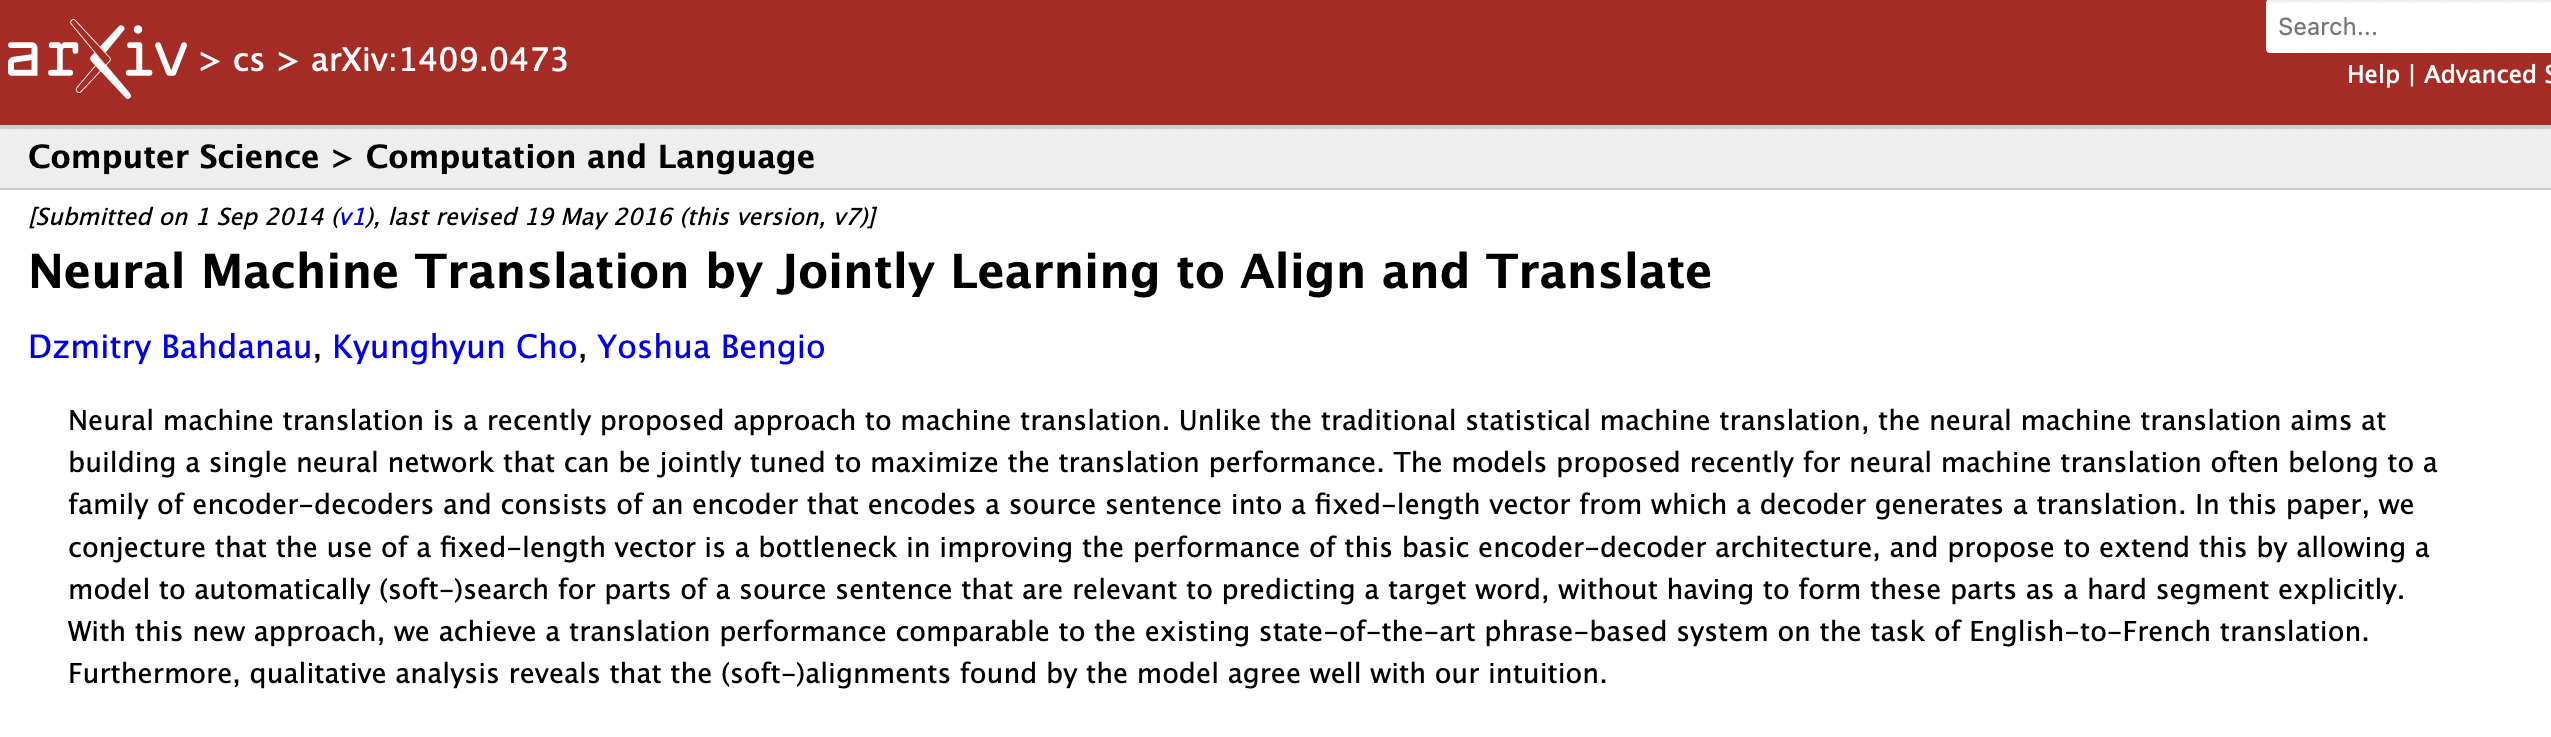
\includegraphics[width=0.85\textwidth]{paper1.png}
\caption{\label{fig:PAPER1}The paper which introduced `attention mechanisms' in 2014.}
\end{figure}


\section{SQL}

For someone starting with learning data science, SQL (pronounced `sequel') can be bit tricky. 
There are two websites which are particularly nice to develop these skills:

\href{https://learnsql.com/blog}{\texttt{Learn SQL}}  \\ 
\href{https://sqlzoo.net/wiki/SQL_Tutorial}{\texttt{SQL Zoo}} 

% /sql-join-examples-with-explanations/
% 


\subsection{Main commands} 

\begin{itemize}
\item \textbf{SELECT}: The SELECT statement is used to retrieve data from one or more tables in a database. You should master using SELECT to filter, sort, and group data using different functions such as WHERE, ORDER BY, and GROUP BY. Here is an example of a SELECT statement:
\begin{quote}
\begin{verbatim}
SELECT column1, column2, column3 FROM table_name WHERE condition; 
\end{verbatim}
\end{quote}
\item In this example, column1, column2, and column3 are the names of the columns that you want to retrieve data from, and table\_name is the name of the table that contains the data. The WHERE clause is optional but is used to specify a condition that must be met in order for the query to retrieve data. Here’s an example that selects all records from a table called `customers' where the customer’s age is greater than or equal to 18:
\begin{quote}
\begin{verbatim}
SELECT * 
FROM customers
WHERE age >= 18;
\end{verbatim}
\end{quote}


\item \textbf{JOIN}: The JOIN statement is used to combine data from two or more tables in a database. You should master using JOIN to retrieve data from multiple tables and specify the type of join (e.g. INNER, LEFT, RIGHT, FULL OUTER) as appropriate.
An INNER JOIN returns only the rows where there is a match between the columns in both tables. Here is an example:
\begin{quote}
\begin{verbatim}
SELECT orders.order_id, customers.customer_name
FROM orders
INNER JOIN customers
ON orders.customer_id = customers.customer_id;
\end{verbatim}
\end{quote}
In this example, the orders table and the customers table are joined using the customer\_id column. The resulting table will only include the order\_id and customer\_name columns where there is a match between the customer\_id columns in both tables.

\item \textbf{LEFT JOIN}: A LEFT JOIN returns all the rows from the left table and the matching rows from the right table. If there is no match in the right table, the result will contain NULL values. Here is an example:
\begin{quote}
\begin{verbatim}
SELECT customers.customer_name, orders.order_id
FROM customers
LEFT JOIN orders
ON customers.customer_id = orders.customer_id;
\end{verbatim}
\end{quote}
In this example, the customers table is the left table and the orders table is the right table. The customer\_id column is used to join the tables. The resulting table will include all the rows from the customers table and the matching rows from the orders table. If there is no match in the orders table, the order\_id column will contain NULL values.



\item \textbf{RIGHT JOIN}: A RIGHT JOIN returns all the rows from the right table and the matching rows from the left table. If there is no match in the left table, the result will contain NULL values. Here is an example:
\begin{quote}
\begin{verbatim}
SELECT customers.customer_name, orders.order_id
FROM customers
RIGHT JOIN orders
ON customers.customer_id = orders.customer_id;
\end{verbatim}
\end{quote}
In this example, the orders table is the left table and the customers table is the right table. The customer\_id column is used to join the tables. The resulting table will include all the rows from the orders table and the matching rows from the customers table. If there is no match in the customers table, the customer\_name column will contain NULL values.



\item \textbf{OUTER JOIN}: An OUTER JOIN in SQL is used to return all the rows from one or both tables, including the non-matching rows. There are two types of OUTER JOINs: LEFT OUTER JOIN and RIGHT OUTER JOIN.
\begin{quote}
\begin{verbatim}
SELECT customers.customer_name, orders.order_id
FROM customers
LEFT OUTER JOIN orders
ON customers.customer_id = orders.customer_id;

* Now RIGHT OUTER JOIN

SELECT customers.customer_name, orders.order_id
FROM customers
RIGHT OUTER JOIN orders
ON customers.customer_id = orders.customer_id;
\end{verbatim}
\end{quote}
In this example, the orders table is the left table and the customers table is the right table. The customer\_id column is used to join the tables. The resulting table will include all the rows from the orders table and the matching rows from the customers table. If there is no match in the customers table, the customer\_name column will contain NULL values. Some databases may not support RIGHT OUTER JOINs, but you can achieve the same result by using a LEFT OUTER JOIN and swapping the order of the tables.


\item \textbf{WHERE}: 
\begin{quote}
\begin{verbatim}
SELECT name, department, salary
FROM employees
WHERE department = 'Sales' AND salary > 50000;
\end{verbatim}
\end{quote}



\item \textbf{GROUP BY}: 
\begin{quote}
\begin{verbatim}
SELECT department, AVG(salary) as avg_salary
FROM employees
GROUP BY department;
\end{verbatim}
\end{quote}


\item \textbf{HAVING}: 
\begin{quote}
\begin{verbatim}
SELECT customer_id, SUM(quantity) AS total_quantity
FROM orders
GROUP BY customer_id
HAVING SUM(quantity) >= 50;
\end{verbatim}
\end{quote}


These are Window functions. 
\item \textbf{HAVING}: 
\begin{quote}
\begin{verbatim}
ROW_NUMBER() \\
SUM()\\
RANK()\\
AVERAGE()\\
Basic query: SELECT column1, column2, ..., ####() OVER (ORDER BY column1)
AS row_num
FROM table_name;
\end{verbatim}
Replace hashes by either four of these like RANK(). 
\end{quote}


\item \textbf{UNION}:  Suppose we have two tables named “customers” and “employees”, both with columns for “name” and “city”. We want to create a list of all people (both customers and employees) who live in New York City. We can use the UNION operator to combine the results of two SELECT statements, one for each table:
\begin{quote}
\begin{verbatim}
SELECT name, city
FROM customers
WHERE city = 'New York'
UNION
SELECT name, city
FROM employees
WHERE city = 'New York';
\end{verbatim}
\end{quote}


\item \textbf{CREATE}:  The CREATE statement is used to create a new database table, view, or other database objects. You should master using CREATE to create new tables, views, and other database objects. Here’s an example of using the CREATE statement in SQL. Suppose we want to create a new table called “customers” with columns for “id”, “name”, “email”, and “phone”. We can use the CREATE statement to do this:
\begin{quote}
\begin{verbatim}
CREATE TABLE customers (
  id INT PRIMARY KEY,
  name VARCHAR(50),
  email VARCHAR(100),
  phone VARCHAR(20)
);

INSERT INTO customers (id, name, email, phone)
VALUES (1, 'John Doe', 'johndoe@example.com', '555-555-1234');
\end{verbatim}
\end{quote}


\item \textbf{INSERT}:  As name suugests
\begin{quote}
\begin{verbatim}
INSERT INTO students (id, name, major, gpa)
VALUES (1234, 'John Doe', 'Computer Science', 3.5);
\end{verbatim}
\end{quote}


\item \textbf{UPDATE}:  As name suugests
\begin{quote}
\begin{verbatim}
UPDATE students
SET major = 'Mathematics', gpa = 3.7
WHERE id = 1234;
\end{verbatim}
\end{quote}


\item \textbf{DELETE}:  This query below would remove the row with an ID of 1234 from the “students” table. The DELETE statement specifies the name of the table we want to delete from, followed by the WHERE clause to specify which rows we want to delete. In this case, we want to delete the row with an ID of 1234, so we specify “WHERE id = 1234”.
\begin{quote}
\begin{verbatim}
DELETE FROM students
WHERE id = 1234;
\end{verbatim}
\end{quote}



% https://levelup.gitconnected.com/13-sql-statements-for-90-of-your-data-science-tasks-27902996dc2b



\end{itemize}

SQL is case insensitive. 

\begin{itemize}
\item \textsc{find second highest salary}:  \texttt{SELECT MAX(SALARY) FROM Employee WHERE SALARY < (SELECT MAX(SALARY) FROM Employee);}
\item \textsc{nth highest salary:} \texttt{Select Salary from EMPLOYEE order by Salary DESC limit n-1,1;} 
\item \texttt{select * from city where population > 100000 and CountryCode="USA"} 
\item \texttt{select * from city where ID="1661"} 
\item \texttt{SELECT NAME FROM CITY WHERE COUNTRYCODE = 'JPN'} 
\item \texttt{SELECT * FROM Student WHERE FirstName NOT LIKE 'A\%'} -- The following query returns the rows in which FirstName do not start with A.
\item \texttt{SELECT * FROM Student WHERE FirstName NOT LIKE '\%d'} -- The following query returns the rows in which FirstName do not end with d.
\item \texttt{select distinct(city) from station where city not REGEXP '\^[AEIOU]' AND city not REGEXP '[aeiou]\$'; } : Query the list of CITY names from STATION that do not start with 
vowels and do not end with vowels. Your result cannot contain duplicates.
\item \texttt{select distinct(city) from station where city not REGEXP '\^[AEIOU]' OR city not REGEXP '[aeiou]\$'; } : Query the list of CITY names from STATION that either do not start with 
vowels or do not end with vowels. Your result cannot contain duplicates.
\item \texttt{SELECT NAME FROM EMPLOYEE ORDER BY NAME ASC;}: Write a query that prints a list of employee names (i.e.: the name attribute) from the Employee table in alphabetical order.
\item \texttt{SELECT NAME FROM EMPLOYEE WHERE SALARY > 2000 AND MONTHS < 10 ORDER BY EMPLOYEE\_ID ASC}: Write a query that prints a list of employee names (i.e. the name attribute) for employees in Employee having a salary greater than  2000 per month who have been employees for less than  10 months. Sort your result by ascending employee-id.
\item \texttt{ALTER TABLE celebs  ADD COLUMN twitter\_handle TEXT;}: Add new column 
\item \texttt{DELETE FROM celebs WHERE twitter\_handle IS NULL;}: Delete rows where one specific column is empty
\item \texttt{SELECT SUM(v) FROM ELEMENTS}: Sum Column $v$ from table ELEMENTS
\item \begin{quote}
\begin{verbatim}
SELECT 
  employee_id,
  last_name,
  first_name,
  salary,
  RANK() OVER (ORDER BY salary DESC) as ranking
FROM employee
ORDER BY ranking
\end{verbatim}
\end{quote}
In this example query, we will show a list of all employees ordered by salary (highest salary first). The report will include the position of each employee in the ranking.
RANK is a function which arranges salary in DESC as ranking. 
\item \begin{quote}
\begin{verbatim}
WITH employee_ranking AS (
  SELECT
    employee_id,
    last_name,
    first_name,
    salary,
    RANK() OVER (ORDER BY salary DESC) as ranking
  FROM employee
)
SELECT
  employee_id,
  last_name,
  first_name,
  salary
FROM employee_ranking
WHERE ranking <= 5
ORDER BY ranking
\end{verbatim}
\end{quote}
Top 5 salary rankings. 
\item 




\item \texttt{CREATE TABLE}: creates a new table,  \texttt{INSERT INTO}: adds a new row to a table, \texttt{SELECT} queries data from a table, 
\texttt{ALTER TABLE} changes an existing table, \texttt{UPDATE}: edits a row in a table, \texttt{DELETE FROM} deletes rows from a table. 
\end{itemize} 

% P is <alias for the source query> and PV is <alias for the pivot table>.



































\section{Basic programming algorithms}

There are different ways to sort a list. Some important ones can be remembered by mneumonic \textbf{ISBMQ}. 
Insertion, Selection, Bubble, Merge, Quick. We denote time and space complexity as $C(\cdot, \cdot)$

\begin{itemize} 
\item Insertion: Start with second element of the list and place it on left or right of first element. Do this loop over elements similarly.  $C(N^2, 1)$
\item Selection: Find minimum of list and place it first (assuming ascending sort). Then focus on remaining and iterate.   $C(N^2, 1)$
\item Bubble: This works by repeatedly swapping the adjacent elements if they are in the wrong order.  $C(N^2, 1)$
\item Merge: Divide and conquer. It divides the input array into two halves, calls itself for the two halves, and then merges the two sorted halves.  The merge(A, p, q, r) is a key process that assumes that A[p..q] and A[q+1..r] are sorted and merges the two sorted sub-arrays into one. $C(N \log N, N$)
\item Quicksort: QuickSort is also a divide and conquer algorithm. It picks an element as a pivot and partitions the given array around the picked pivot. There are many different versions of quickSort that pick pivot in different ways. $N \log N, \log N$
\end{itemize} 



\section{Codility Exercises Solutions}

\textsc{Question 1:} \href{https://app.codility.com/programmers/trainings/1/longest_password/}{LongestPassword (see here)} \\
\textsc{Solution 1:} 


\begin{mdframed}[backgroundcolor=celadon!6]
\lstinputlisting[language=Python]{codes/password.py}
\end{mdframed}

\textsc{Question 2:} \href{https://app.codility.com/programmers/lessons/1-iterations/binary_gap/}{Binary Gap (see here)} \\
\textsc{Solution 2:} 

\begin{mdframed}[backgroundcolor=celadon!6]
\begin{lstlisting}[language=Python]
def solution(N):
    return len(max(format(N, 'b').strip('0').split('1'))) 
\end{lstlisting}
   \end{mdframed} 
   
   
   
   % Fast API: https://www.datacamp.com/tutorial/introduction-fastapi-tutorial
   


\section{Interview questions}

\begin{enumerate}

\item Q1: How to improve your model performance?  \\
\textsc{Answer:} Some methods are -- use validation methods, add more data, apply feature engineering techniques (normalization, imputation etc.), compare multiple algorithms, hyperparameter tuning 

\item Q2: What is difference between standardization and log transformation. \\
\textsc{Answer:} Standardization is the process of putting different variables on the same scale. This process allows you to compare scores between different types of variables. Typically, to standardize variables, you calculate the mean and standard deviation for a variable. Log transformation is a data transformation method in which it replaces each variable $x$ with a $log(x)$. Log-transform decreases skew in some distributions, especially with large outliers. But, it may not be useful as well if the original distribution is not skewed. Also, log transform may not be applied to some cases (negative values), but standardisation is mostly always applicable except $\sigma = 0$. 

\item Q3: How to deal with unbalanced binary classification? \\
\textsc{Answer:} In a classification task, there is a high chance for the algorithm to be biased if the dataset is imbalanced. An imbalanced dataset is one in which the number of samples in one class is very higher or lesser than the number of samples in the other class. 
To counter such imbalanced datasets, we use a technique called up-sampling and down-sampling. In up-sampling, we randomly duplicate the observations from the minority class in order to reinforce its signal. The most common way is to resample with replacement. In down-sampling, we randomly remove the observations from the majority class. Thus after up-sampling or down-sampling, the dataset becomes balanced with the same number of observations in each class.

\end{enumerate}
















	
	\newpage
	\addcontentsline{toc}{section}{References}
	\bibliographystyle{utphys}
	\bibliography{ref.bib}
\end{document}
